\section{Material und Methoden}

In diesem Kapitel werden das zu Grunde liegende Material -- die Grabungsfotos -- und die darauf angewendete Software vorgestellt. Im Anschluss wird die Verarbeitung der Fotos im Detail beschrieben. 
Diese gliedert sich in zwei Teilbereiche: Die Tafeldetektion und die Texterkennung (OCR\footnote{\textit{Optical Character Recognition}}). Die Tafeldetektion wiederum ist in die eigentliche Erkennung sowie das Ausschneiden der Tafeln aus dem Gesamtbild unterteilt. Für beide Arbeitsschritte gibt es je zwei Varianten.
%eigentliches Material: Fotos!
\subsection{Fotos}
Der Gegenstand dieser Arbeit sind 1.453 Fotos, die während der Grabungen auf dem Kapitol in Rom in den Jahren 2011-2014 entstanden sind. Die Fotos haben eine Auflösung von 3264 x 2448 Pixeln und liegen im JPG-Format vor. Teilweise sind die exif-Daten\footnote{Exchangeable Image File Format, das Standardformat für Metadaten in Bilddateien\cite{exif}} vorhanden, die von der Kamera erzeugt wurden. Sie beinhalten das Datum, das Kameramodell (Nikon Coolpix L19), die Belichtungsdauer und den ISO-Wert für die Lichtempfindlichkeit des Fotosensor. Weitere Metadaten -- Datum, Ort, das Kürzel für die Grabung sowie weitere Anmerkungen -- befinden sich auf Tafeln, die auf einigen der Fotos zu sehen sind. Das Datum auf der Tafel und das in den exif-Daten weichen teilweise um mehrere Tage voneinander ab.
Bei den Tafeln, die auf den Grabungsfotos zu sehen sind, handelt es sich um Schiefertafeln mit einem Holzrahmen, die mit Kreide beschriftet wurden (Vgl. Abb \ref{fig:einfachetafel}). Die Detektion der Tafeln beruht auf folgenden Faktoren: (1) Die Tafeln haben grundsätzlich eine rechteckige Form. (2) Durch die Breite des Rahmens können bis zu zwei Rechtecke erkannt werden, ein inneres und ein äußeres. (3) Der Rahmen ist hell und die Schreibfläche dunkel, es besteht ein starker Kontrast.
\begin{figure}[!h]
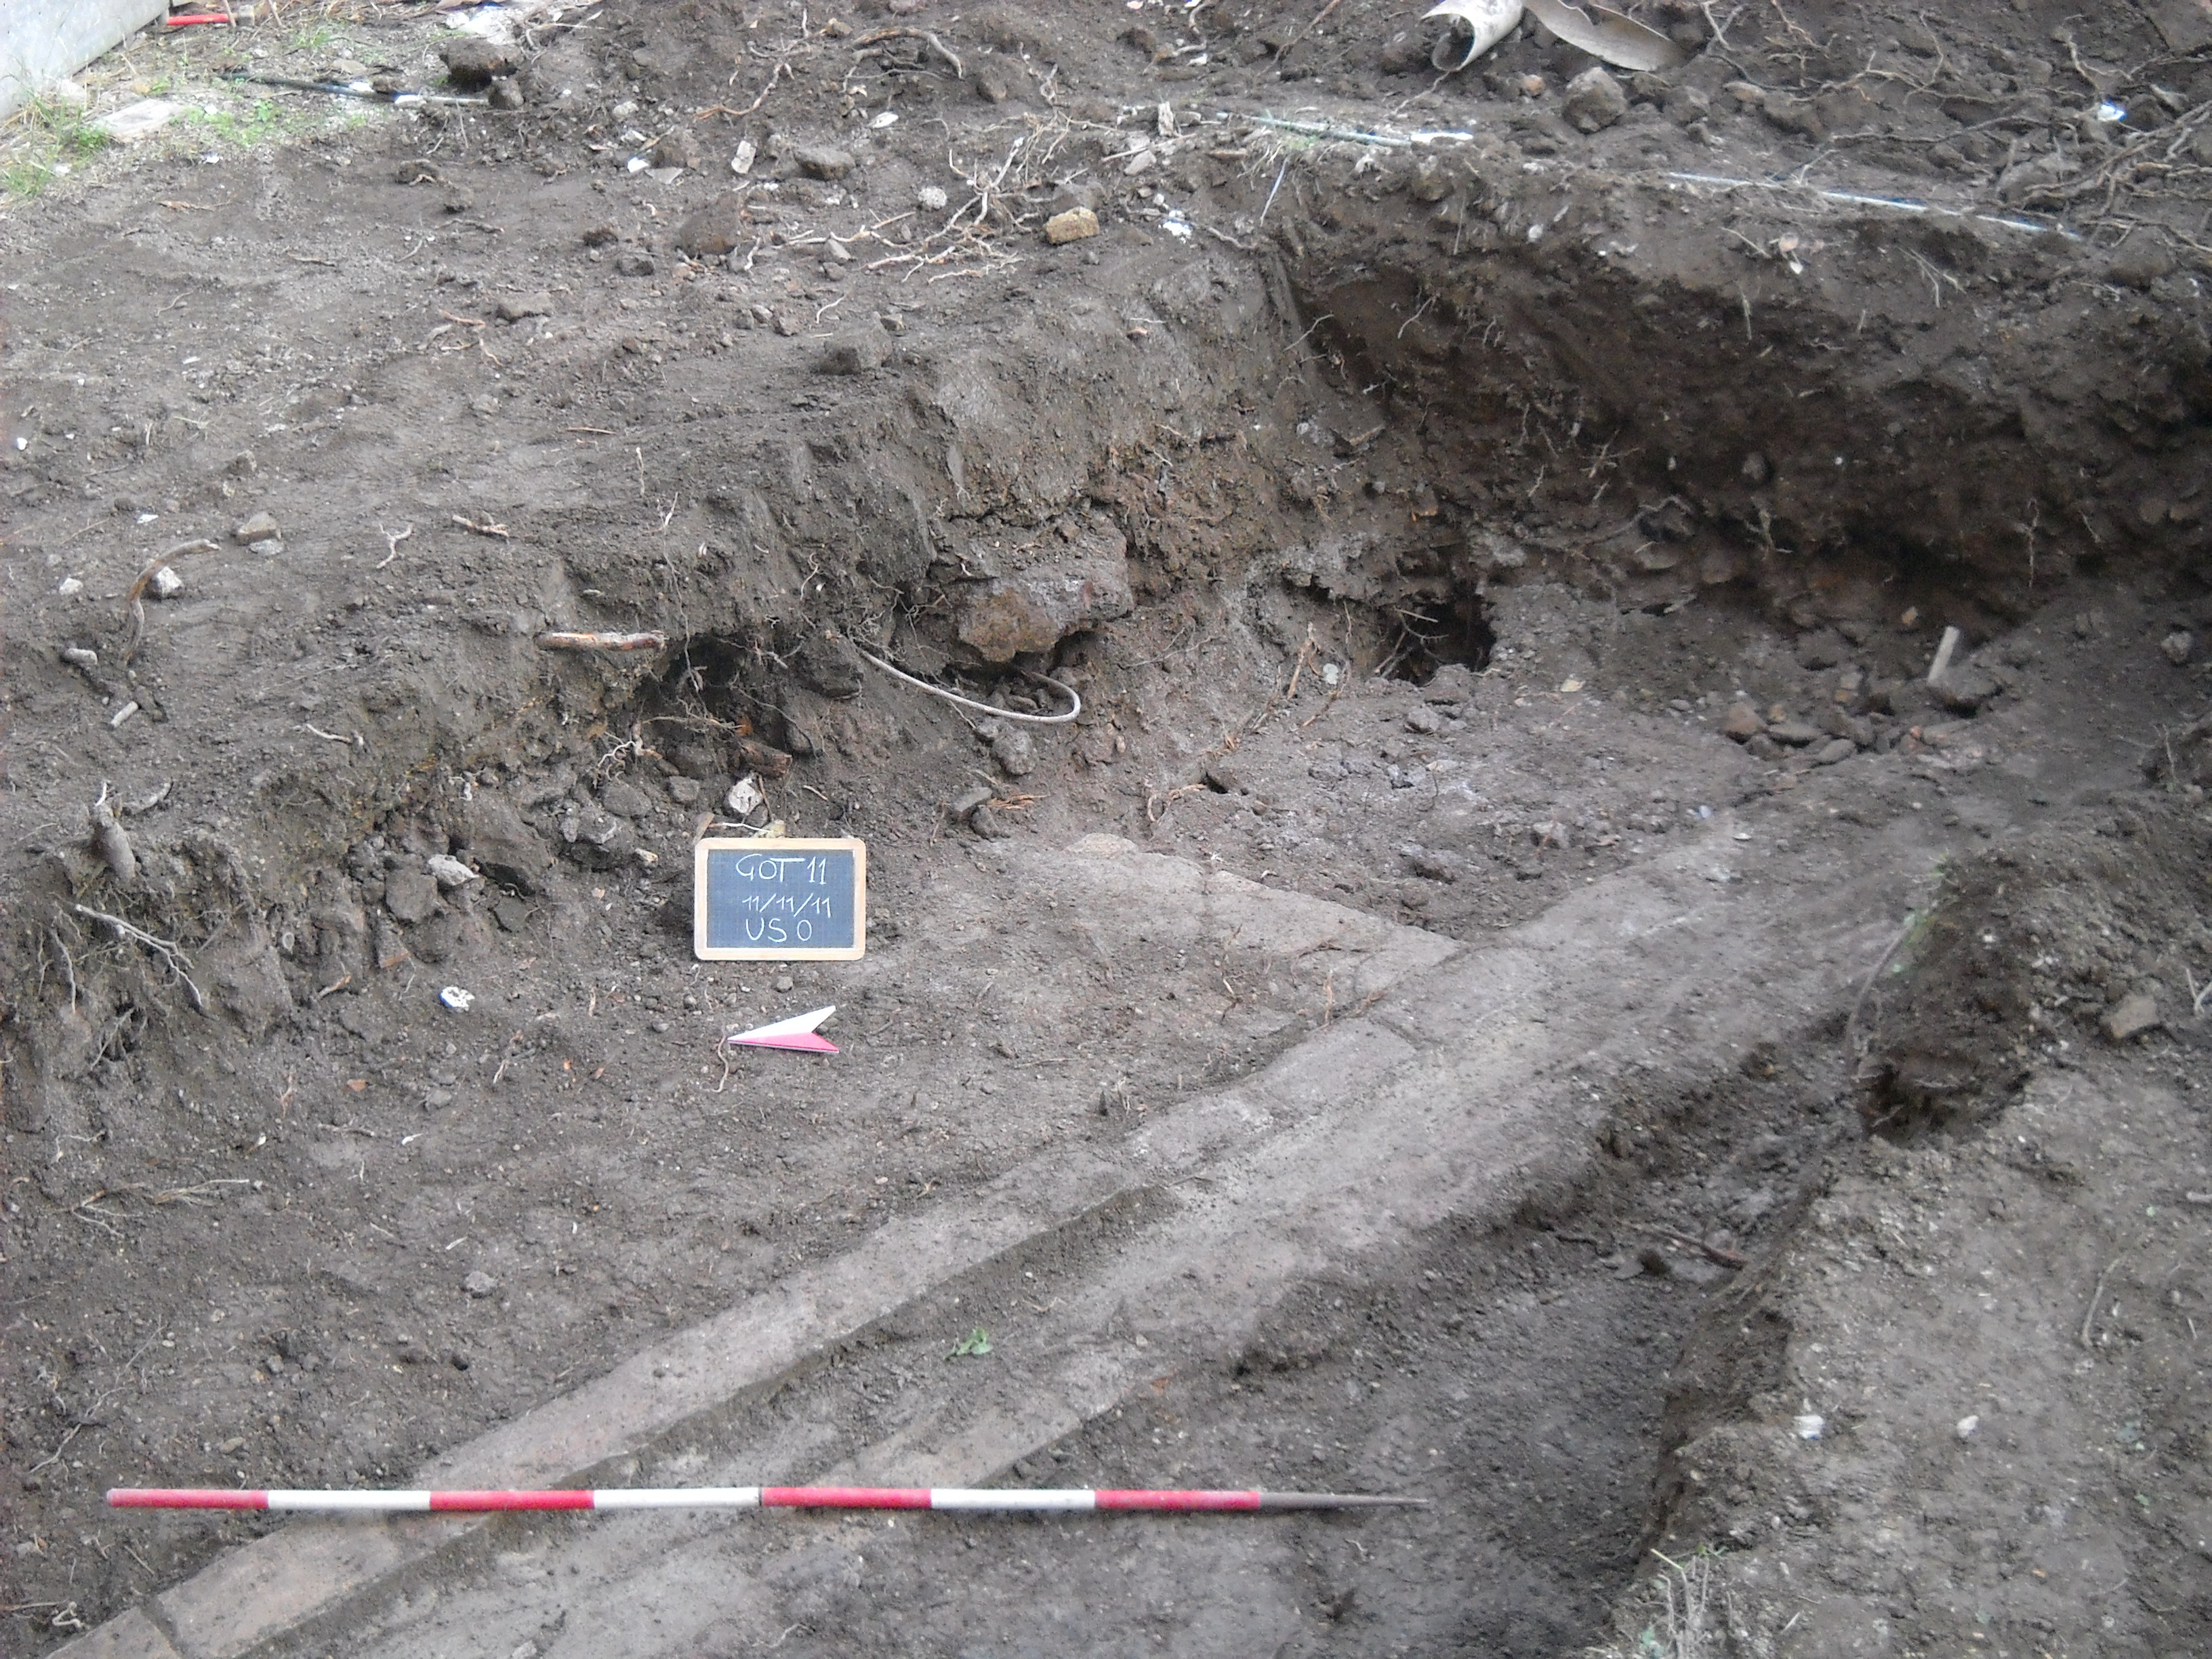
\includegraphics[width =0.5\textwidth]{catacom_1020.JPG}
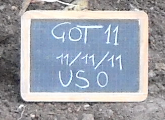
\includegraphics[width=0.5\textwidth]{catacom_1020_cutout.png}
\caption{Beispiel eines Fotos der verwendeten Tafel. GOT bezeichnet die Kampagne, darunter folgt das Datum. US (\textit{unità stratigrafica}) bezeichnet die stratigrafische Einheit.}
\label{fig:einfachetafel}
\end{figure}
Die im Beispielbild gezeigte Tafel stellt  ein Idealbild dar: Die Tafel nimmt einen relativ großen Teil des Originalbildes ein. Sie ist frontal vor der Kamera positioniert. Die Beleuchtung ist gut und indirekt. Keines der weiteren Bildelemente verdeckt die Tafel.
Diese Beschreibung impliziert schon die Problemfelder, die bei der Detektion beachtet werden müssen:
\begin{enumerate}
\item Die Tafel ist unter Umständen rotiert (Abb \ref{fig:schwierigetafel}).
\item Die Distanz der Tafel zur Kamera und damit ihre Größe im Bild kann stark variieren.
\item Der Rahmen der Tafel kann teilweise verdeckt oder anderweitig durch Gegenstände überlagert sein (Vgl. Abb \ref{fig:schwierigetafel}).
\item Ein geringer Kontrast des Hintergrunds zum Tafelrahmen kann die Detektion erschweren. %(Vgl. Abb \ref{fig:schwierigetafel})
\item Unregelmäßigkeiten im Rahmen, die auf grobe Verarbeitung oder Abnutzung zurückzuführen sind, können die Detektion erschweren.
\item Die Beleuchtung kann zu Problemen führen. Grundsätzlich sind alle Fotos hell und gut ausgeleuchtet, direktes Licht kann sich aber negativ auf die Kontraste auswirken.
\item Weitere Gegenstände, die den Spezifika der Tafeln entsprechen, können im Bild vorhanden sein.
\end{enumerate}
\begin{figure}[!h]
\centering
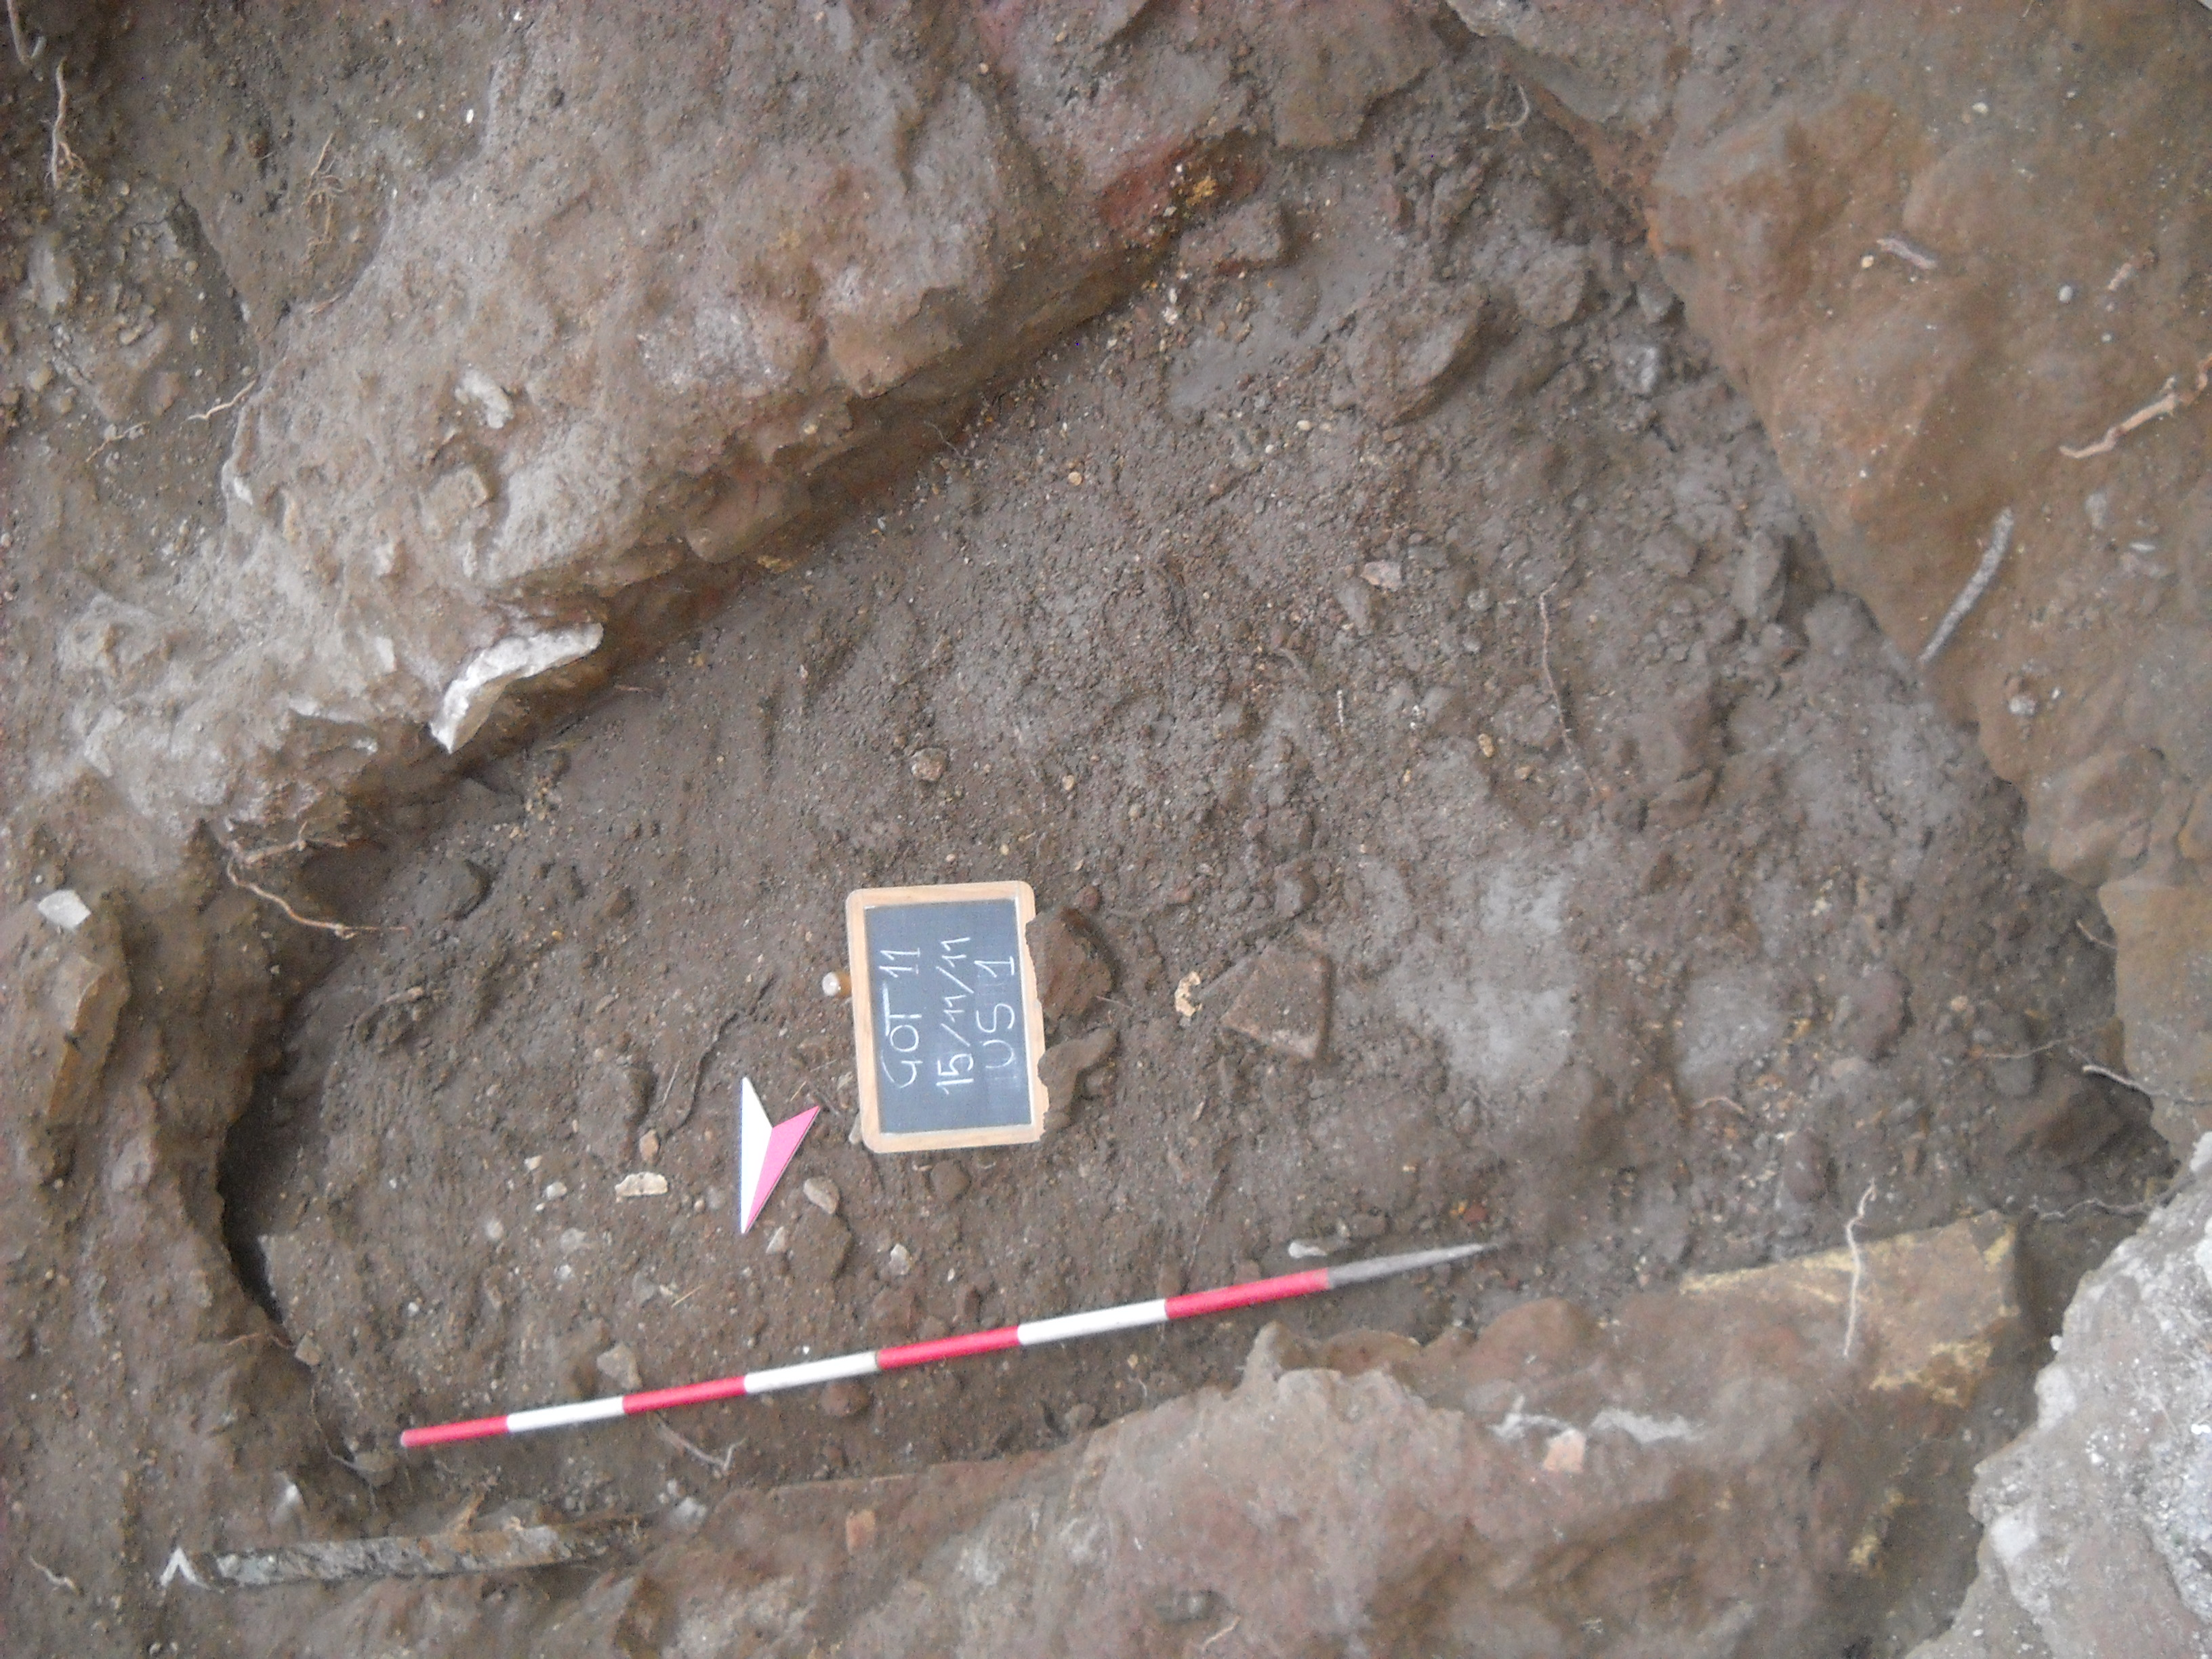
\includegraphics[width =0.5\textwidth]{catacom_1061_schwierige_tafel.JPG}
%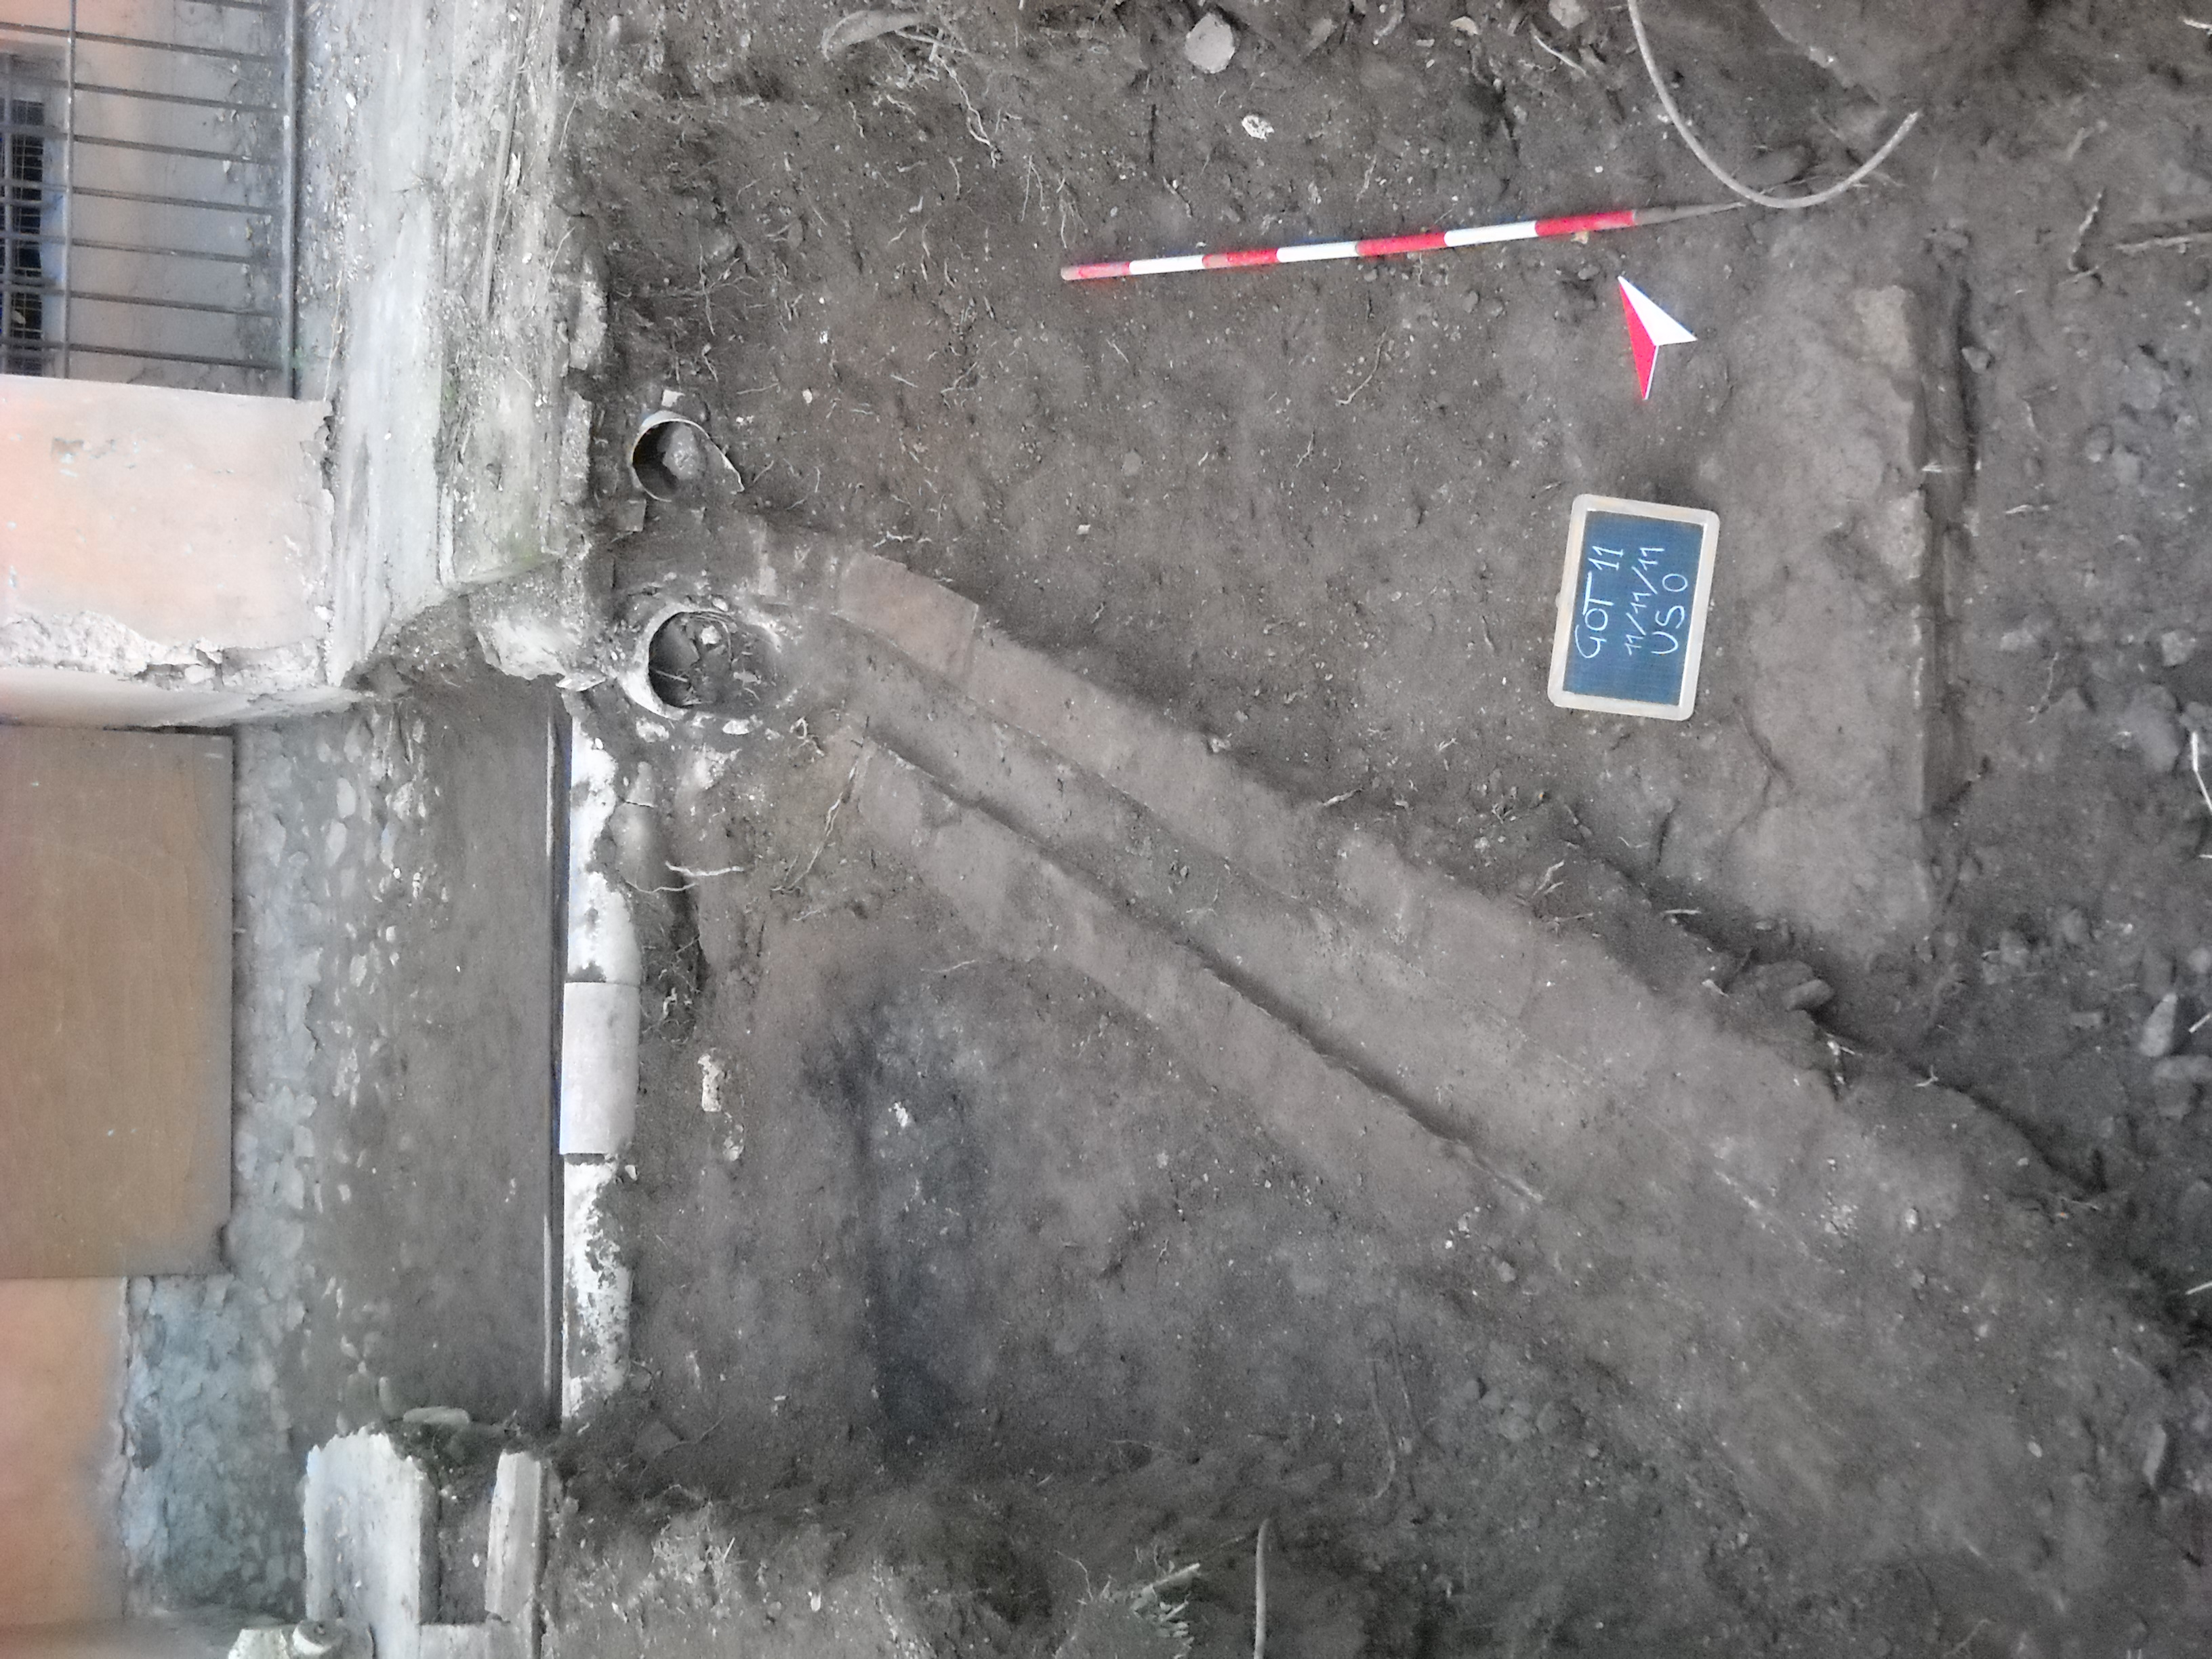
\includegraphics[width =0.5\textwidth]{catacom_1023.JPG}
\caption{Problematische Tafeln: Rotation und teilweise verdeckter Rahmen.}
\label{fig:schwierigetafel}
\end{figure}
%Teilweise werden die hier genannten Probleme auch bei der Texterkennung wieder relevant. Auf diese und auf weitere wird an geeigneter Stelle zurückgegriffen.

\subsection{Software}

Der Programmcode ist in Python (Version 3.8) geschrieben. Verwendet werden die \textit{packages} Numpy (1.19.5) und vor allem OpenCV(4.4.0.44). Die Texterkennung arbeitet mit PyTesseract (0.3.7).

\subsection{Tafeldetektion}

Der folgende Abschnitt befasst sich mit der ersten Teilaufgabe dieser Arbeit: Der Detektion der Tafeln auf den Grabungsfotos. Hier werden mehrere Ansätze vorgestellt, die im Laufe der Auseinandersetzung mit dem Thema erprobt wurden: die Tafeldetektion mittels CNNs und mittels klassischer Computer Vision über die Detektion von Konturen.

\subsubsection{CNN-basierter Ansatz}

\subsubsection{Kontur-basierter Ansatz}

\verb|Cv2.Contours| basiert auf einem Algorithmus, der Punkte gleicher Farbe und Intensität umrandet \cite{findcontours}. Das Resultat ist eine Liste von Punkten, die ein geschlossenes Polygon ergeben. Die gefundenen Konturen können mit einer Hierarchie versehen werden, bei der Konturen, die sich innerhalb anderer Konturen befinden, als deren \glqq Kinder\grqq gelten. Das Verfahren ist darauf ausgelegt, auf binäre Bilder angewendet zu werden. Die Implementierung in OpenCV unterscheidet in Nullwerte und Nicht-Nullwerte \cite{opencvcontours}. Nicht-binäre Bilder werden dadurch automatisch binarisiert. Für die Erzielung optimaler Ergebnisse kommt dem Binarisierungsverfahren eine große Bedeutung zu.
Auf Basis dieses Algorithmus lässt sich Detektionsverfahren aufbauen, das Objekte, die sich vom Hintergrund der Bilder abheben, zu erkennen. Die Herausforderung besteht, nach diesem Ansatz, in zwei Punkten: Erstens muss die Binarisierung so erfolgen, dass eine möglichst saubere Trennung von Vordergrund (Objekten) und Hintergrund (vor allem Erde) der Bilder stattfindet und zweitens müssen aus den gefundenen Vordergrundobjekten diejenigen ausgewählt werden, die als Tafeln in Frage kommen. Bei der Binarisierung haben sich zwei Wege als praktikabel herausgestellt, die im Folgenden beide präsentiert werden sollen. Diese Ansätze werden im Folgenden als adaptiver und als iterativer Ansatz bezeichnet. Im Flowchart sind die Abläufe der Rechtecksdetektion dargestellt (Vgl. Abb.\ref{fig:flowrectdetect}).
\begin{figure}[h!]
\centering
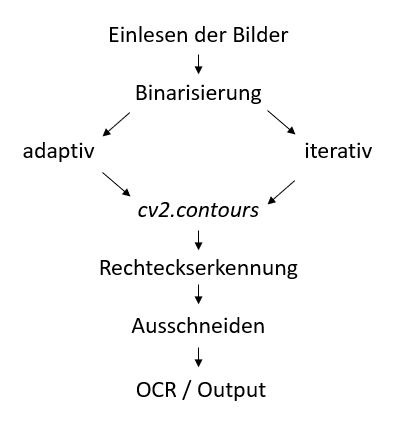
\includegraphics[width =0.5\textwidth]{flowchart_cont.PNG}
\caption{Flowchart Rechteckserkennung: Die Binarisierung erfolgt durch einen der beiden möglichen Ansätze. Auf dieser Basis wird die eine Konturerkennung durchgeführt. Aus diesen Konturen werden die Rechtecke ausgewählt und aus dem Gesamtbild ausgeschnitten. Es folgt die weitere Verarbeitung.}
\label{fig:flowrectdetect}
\end{figure}

\subsubsection*{Adaptive Binarisierung}

Das einfachste Verfahren der Binarisierung eines Bildes besteht darin, einen Grenzwert festzulegen. Dieser muss auf der Spanne der Farbwerte, also zwischen 0 und 255 liegen.  Farbwerte unterhalb dieses Grenzwertes werden zu Nullen, Farbwerte darüber zu Einsen. Das Ergebnis ist ein Schwarz-Weiß-Bild. Bei komplexen Szenerien, wie den Grabungsfotos, ist dieses Verfahren jedoch zu einfach. So kann ein Foto beispielsweise stark unterschiedliche Beleuchtung, wie direktes Sonnenlicht und Schatten, enthalten. Eine Differenzierung innerhalb dieser Zonen ist so nicht möglich (Vgl. Abb. \ref{fig:threshold}).\\
\begin{figure}[h!]
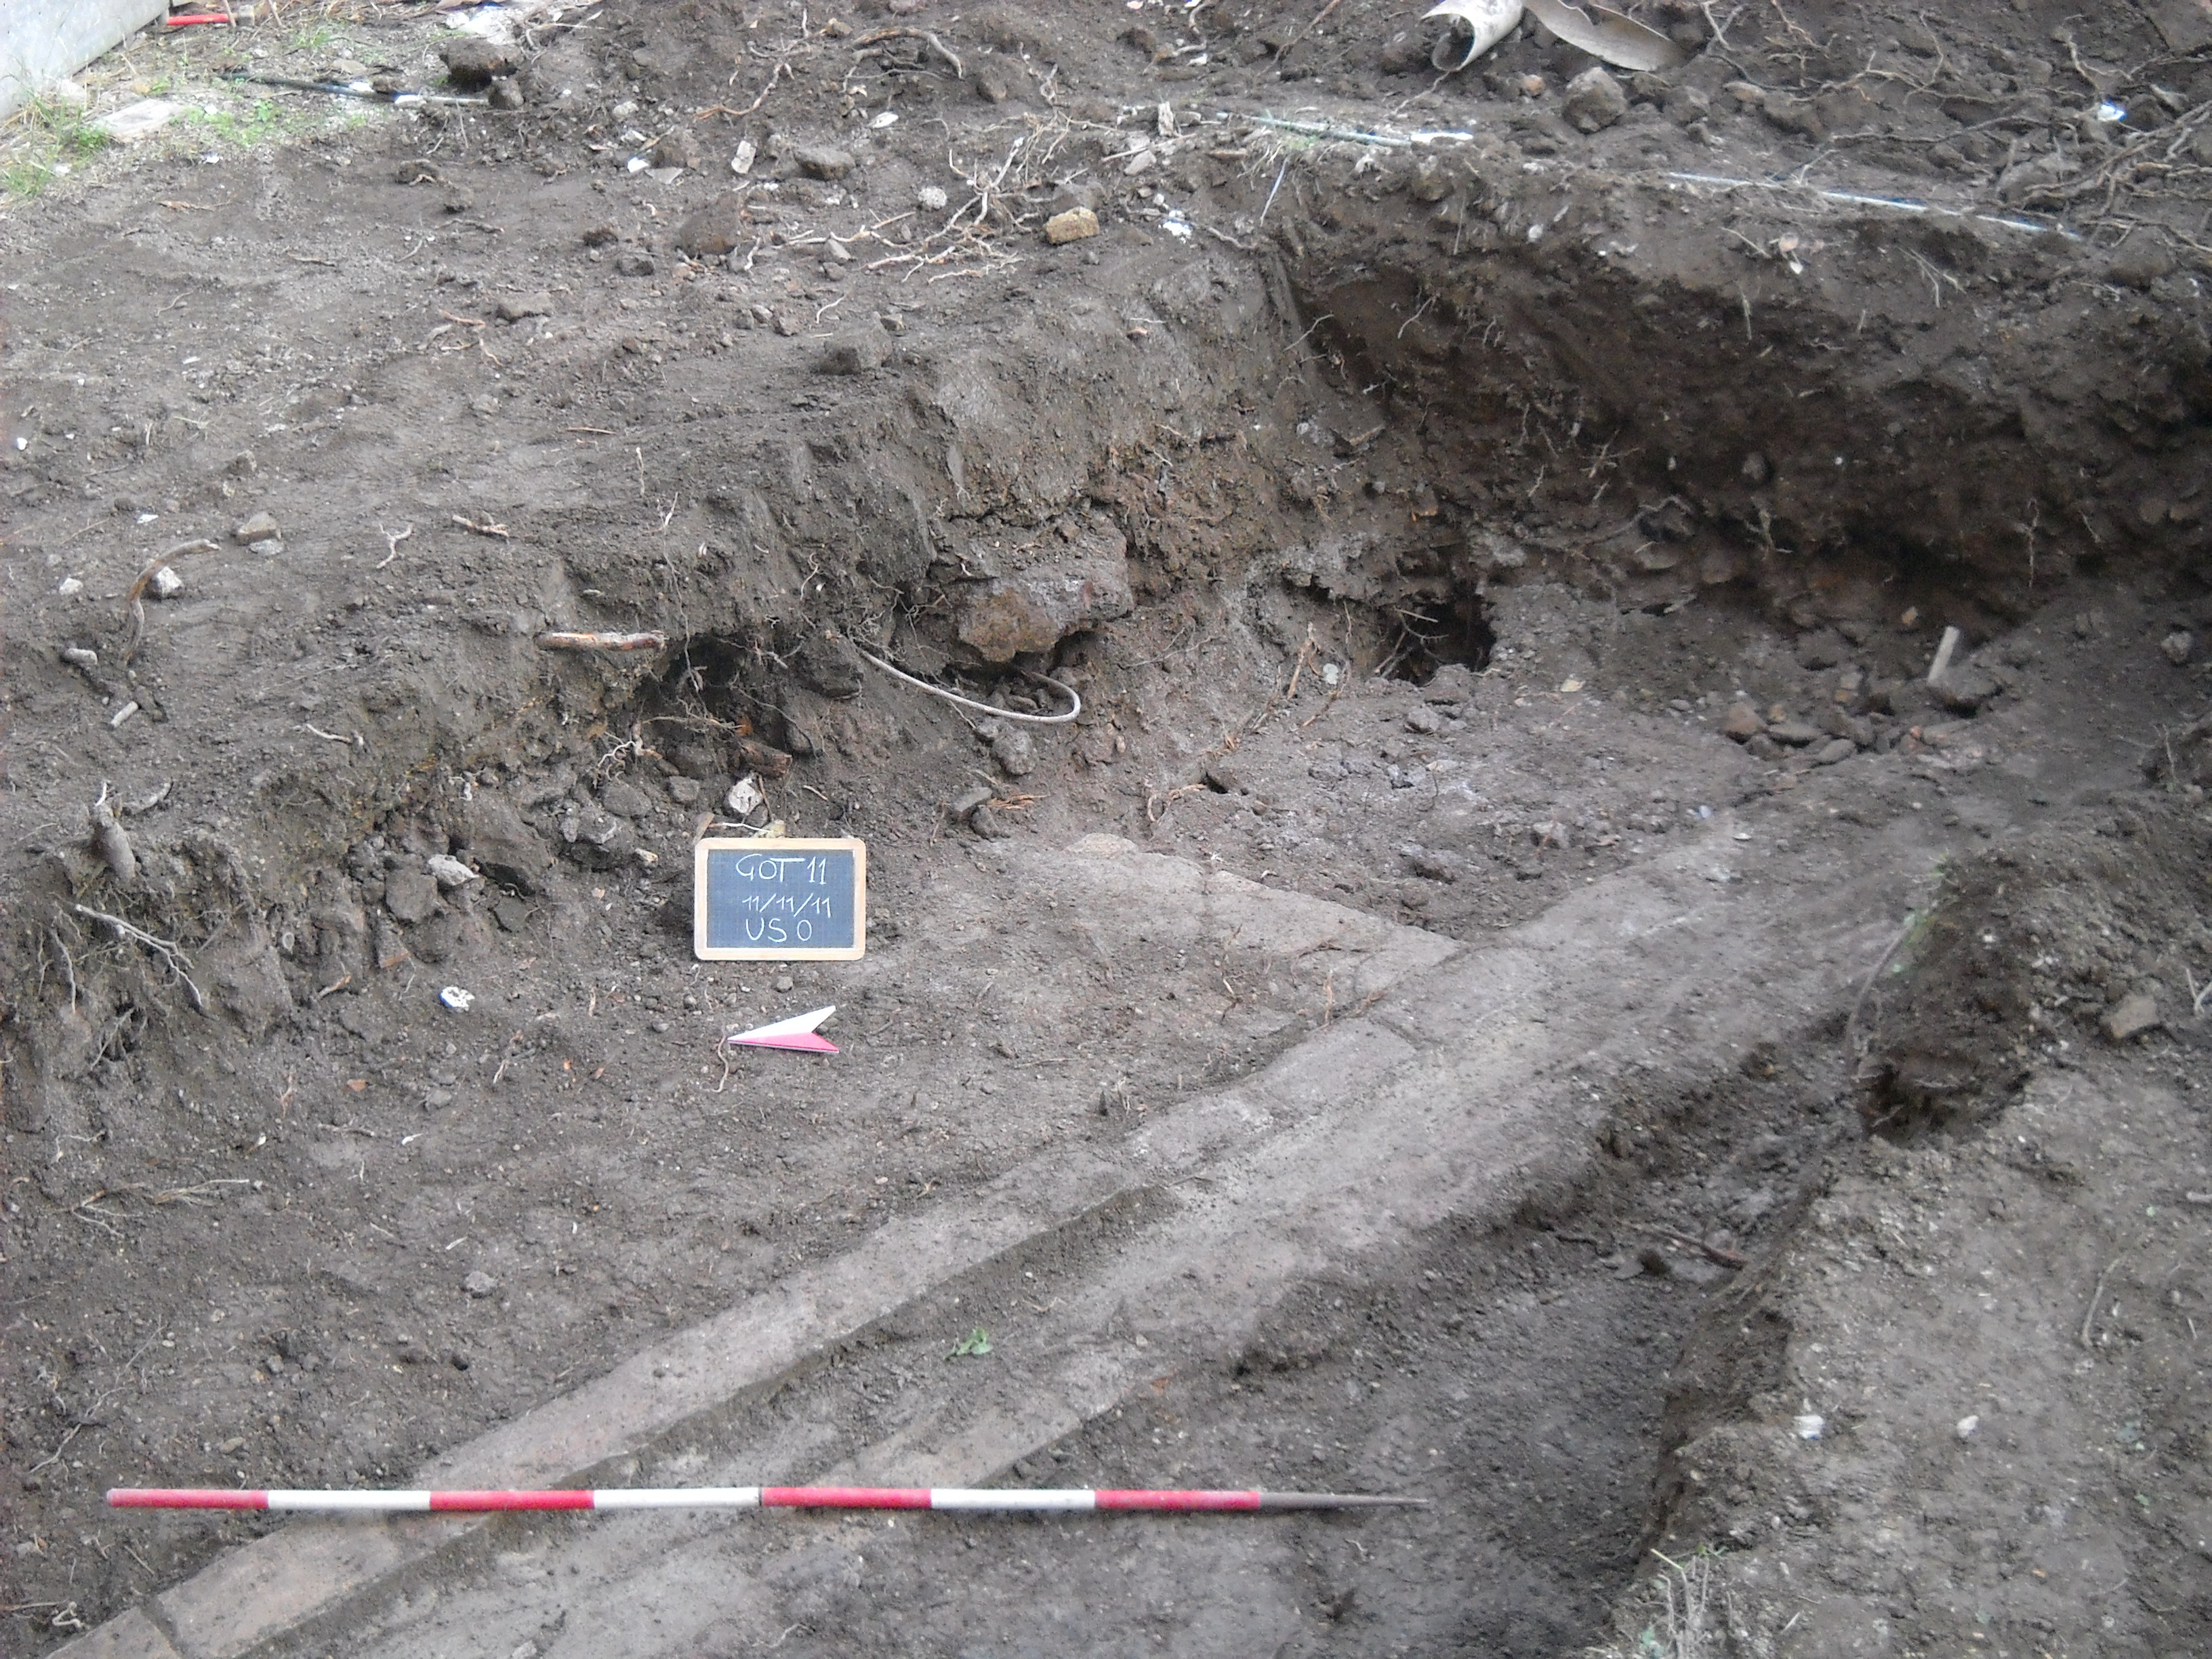
\includegraphics[width =0.5\textwidth]{catacom_1020.JPG}
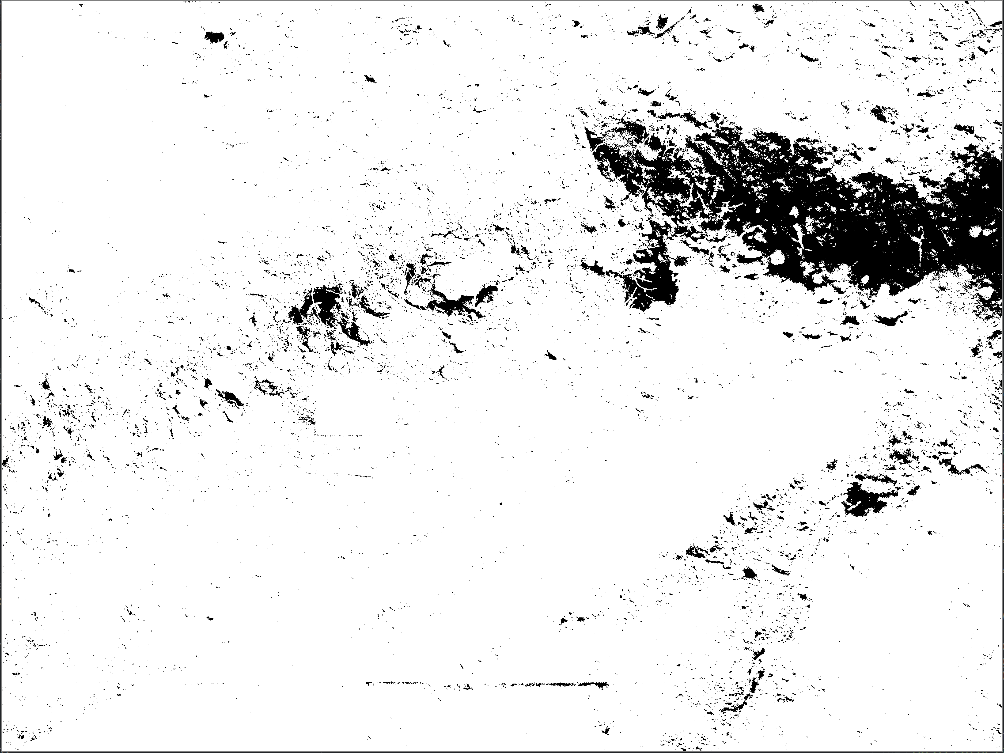
\includegraphics[width =0.5\textwidth]{thresh60.png}
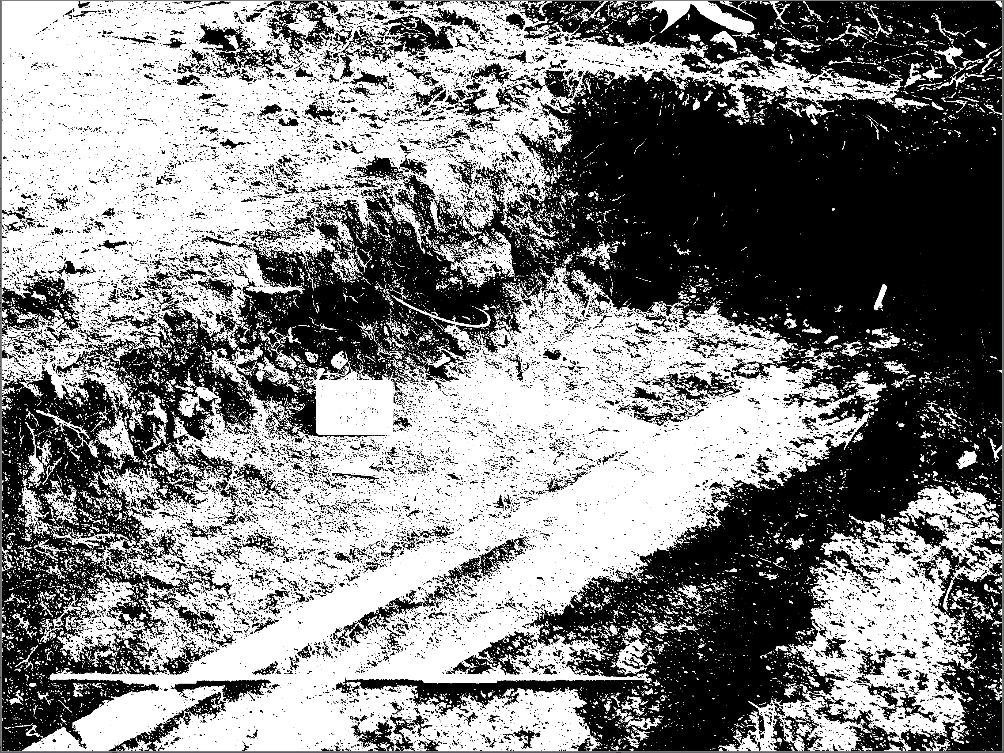
\includegraphics[width =0.5\textwidth]{thresh125.png}
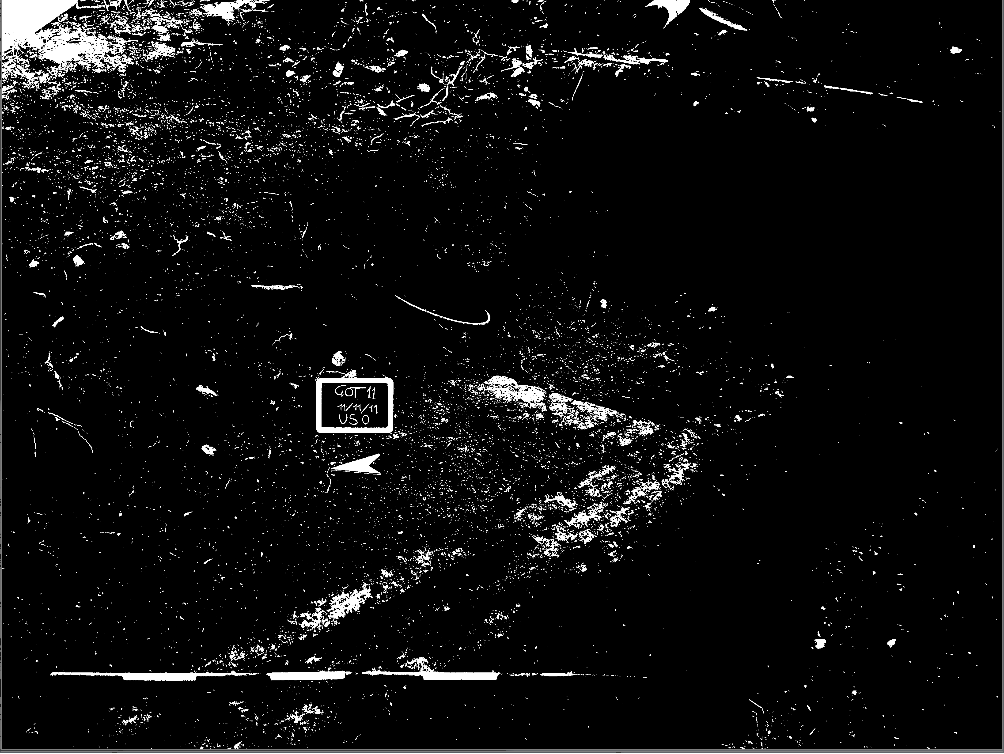
\includegraphics[width =0.5\textwidth]{thresh185.png}
\caption{Grabungsfoto im Original (o.l.), mit niedrigem (60, o.r.), mittlerem (125, u.l.) und hohem (185, u.r.) Grenzwert.}
\label{fig:threshold}
\end{figure}
Daher wird für den ersten Ansatz ein adaptiven Thresholds \cite{opencvadaptivethresholdopencvadaptivethreshold}) gewählt: Statt global, über das gesamte Bild, einen Grenzwert festzulegen, können lokale Grenzwerte errechnet werden. Die Größe des lokalen Ausschnittes sowie das exakte Verfahren können dabei frei gewählt werden. In diesem Fall wird für die Binarisierung ein Gauss-Verfahren auf einen Kernel von 11 x 11 Pixeln angewendet. Die Beleuchtung oder Farbunterschiede innerhalb des Bildes können so ausgeglichen werden (Vgl. Abb. \ref{fig:adaptivethreshold}).
\begin{figure}[h!]
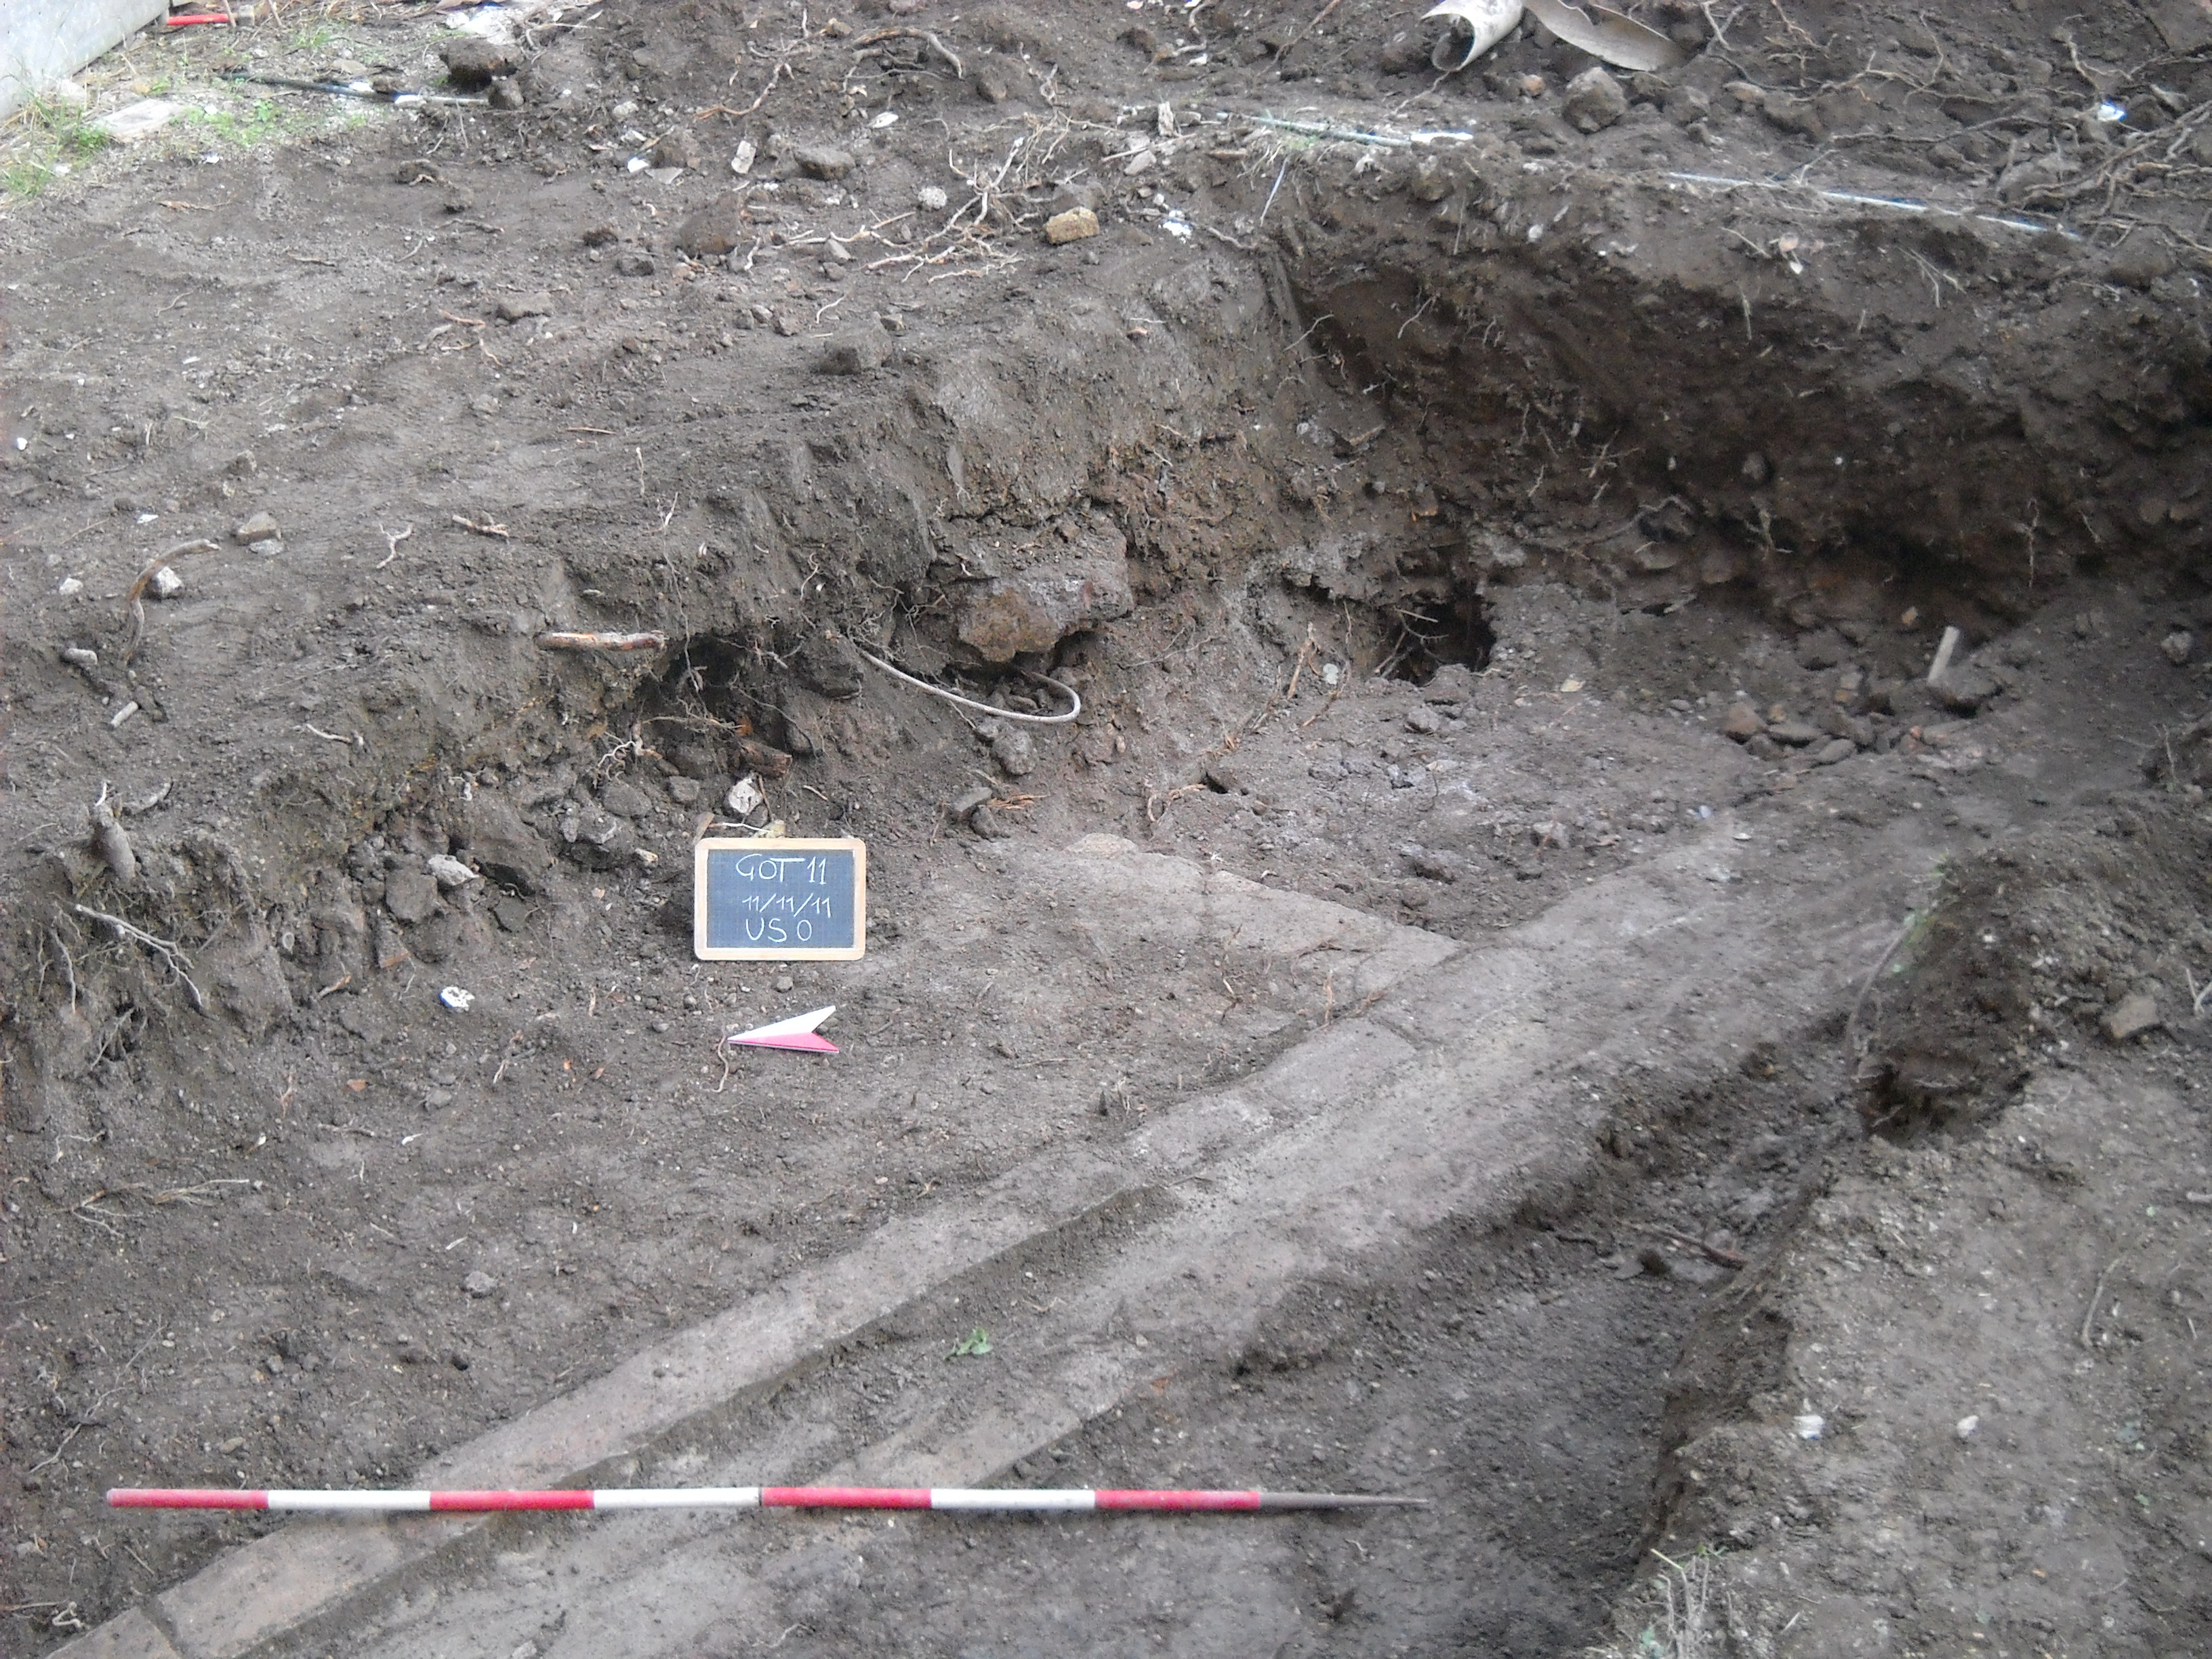
\includegraphics[width =0.5\textwidth]{catacom_1020.JPG}
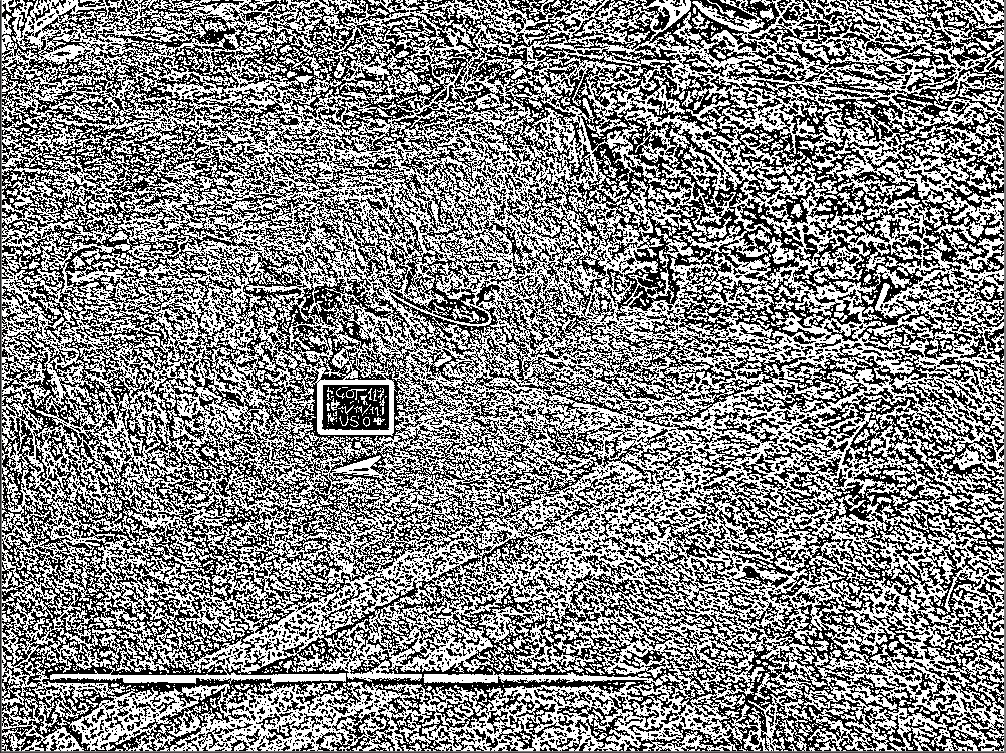
\includegraphics[width =0.5\textwidth]{adaptivethreshold.png}
\caption{Grabungsfoto im Original sowie mit adaptivem Threshold.}
\label{fig:adaptivethreshold}
\end{figure}
Vor der Binarisierung wird das Bild in ein Graustufenbild umgewandelt und verkleinert\footnote{Genauer: Der längere Bildrand wird auf 1000 Pixel reduziert, der kürzere entsprechend angepasst. Die Grabungsfotos haben, wie bereits erwähnt, eine Auflösung von 3264 x 2448 Pixeln. Es findet also eine Reduktion auf ca. $\frac{1}{10}$ der Fläche statt. Bilder kleiner als 1000 Pixel würden theoretisch auf 1000 Pixel vergrößert werden. Da für die hier beschriebenen Prozesse und vor allem für die Texterkennung später aber eine gewisse Bildqualität erforderlich ist, ist von diesem Fall nicht auszugehen.}. Das verbessert die Genauigkeit der Detektion und verringert die zu verarbeitende Datenmenge, wodurch eine Beschleunigung des Prozesses zu erwarten ist. %Die Verkleinerung des Bildes ist allerdings ein Prozess, der später rückgängig gemacht werden muss, um Datenverlust bei der Texterkennung zu verhindern.

\subsubsection*{Iterative Binarisierung}

%Die adaptive Binarisierung bringt einige Nachteile mit sich. So ist hier die Erkennung von Falsch-Positiven relativ hoch. Die Konturen werden auf einem verkleinerten Bild gesucht und müssen später auf Originalgröße skaliert werden, was ein verlustbehafteter Prozess ist.
Die Grundidee der iterativen Binarisierung besteht darin, das Bild mit einem globalen Grenzwert zu binarisieren. Die Problematik davon besteht darin, das bei großen Beleuchtungsunterschieden oder sehr hellen oder dunklen Objekten auf dem Bild ganze Bereiche durch den Grenzwert von der weiteren Bearbeitung ausgeschlossen werden. Der iterative Ansatz sieht daher vor, den Grenzwert von 20 auf 200 in Fünferschritten zu erhöhen. Dadurch entstehen pro Foto 37 binäre Bilder, auf die die Konturenerkennung angewendet werden kann. Auf jedem dieser Bilder können mehrere mögliche Tafeln erkannt werden\footnote{Die eigentliche Tafelerkennung wird erst im folgenden Abschnitt beschrieben. Da die dort gewonnenen Informationen nicht, wie beim adaptiven Ansatz, an das Hauptprogramm übergeben, sondern innerhalb der Funktion des iterativen Ansatzes weiter verarbeitet werden, ist hier ein Vorgriff nötig.}. Der nächste Schritt besteht also darin, aus diesen möglichen Tafeln die auszuwählen, die am wahrscheinlichsten tatsächlich eine ist. Dazu wird eine Grundannahme getroffen: In dem dem Bereich, in dem auf den meisten der 37 Bilder eine Tafel vermutet wird, befindet sich tatsächlich eine Tafel. Alle anderen werden als Falsch-Positive betrachtet. Diese Annahme beruht auf zwei Faktoren: Erstens hat sich gezeigt, dass Objekte, die keine Tafeln sind, aber als solche erkannt werden können -- z.B. Fenster, Türen oder Plakate -- nur unter wenigen Grenzwertes als solche eingeordnet werden. Das liegt unter anderem daran, dass die Tafeln einen hellen Holzrahmen und eine dunkle Innenfläche haben, was zu einem starkem Kontrast führt, der auf vielen Stufen des Grenzwertes erhalten bleibt\footnote{Die Tafeln verfügen damit über eine Eigenschaft, die auch beim Einsatz von AR-Markern genutzt wird: Starke hell-dunkel Kontraste beschleunigen und vereinfachen die Detektion \cite[p.~45]{armarker}}. Außerdem werden durch eben diesen Rahmen in mittleren Grenzwert-Bereichen die Tafeln oft zweimal erkannt: Einmal an der Außenkante und einmal an der Innenkante des Rahmens. Dadurch häuft sich die Detektion möglicher Tafeln in diesem Bereich.
Basierend auf dieser Annahme wird auf alle möglichen Tafeln immer paarweise die \verb|intersection over union| angewendet. Dieser Algorithmus basiert auf dem Jaccard-Koeffizienten zur Berechnung der Ähnlichkeit zweier Mengen \cite{intersectionoverunion}. Der Koeffizienten wird errechnet, indem die Schnittmenge durch die Vereinigungsmenge geteilt wird. Das Ergebnis liegt zwischen 0 und 1. Je mehr es sich der 1 annähert, desto ähnlicher sind die Mengen. Diese Berechnung lässt sich auch auf die Rechtecke, mit denen die möglichen Tafeln verortet werden, anwenden (Vgl. Abb. \ref{fig:jaccard}).

\begin{figure}[h!]
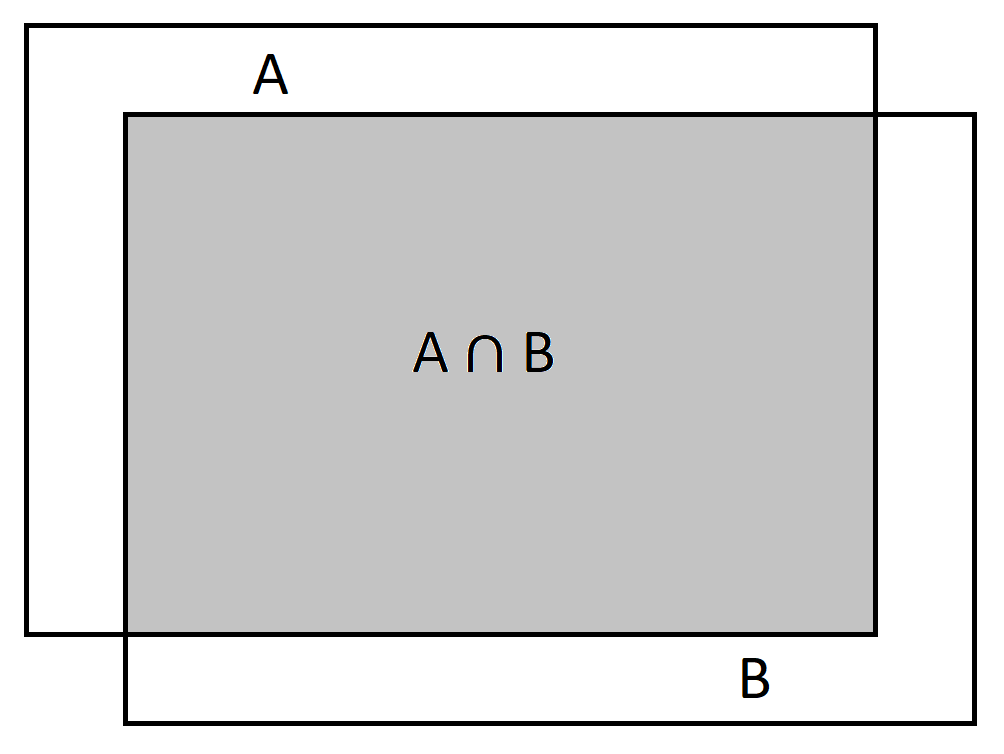
\includegraphics[width =0.5\textwidth]{schnittmenge.png}
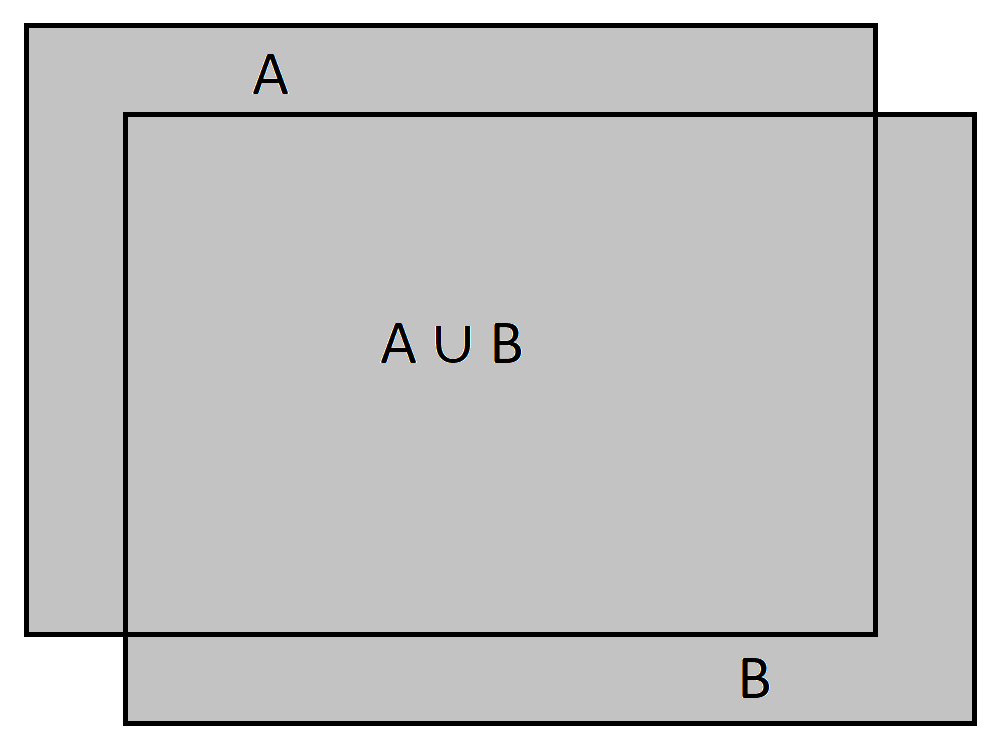
\includegraphics[width =0.5\textwidth]{vereinigungsmenge.png}
\caption{Schnittmenge und Vereinigungsmenge von Rechtecken. Der Jaccard-Koeffizient wird durch die Division der beiden Flächen bestimmt.}
\label{fig:jaccard}
\end{figure}

Zwei Rechtecke galten dann als hinreichend ähnlich, wenn der Jaccard-Koeffizient über 0.9 lag. Jedes Mal, wenn ein Rechteck im Vergleich mit einem anderen diesen Wert erzielt, wird für das Rechteck ein Zähler erhöht. Das Rechteck, welches am Ende der Vergleiche den höchsten Wert in diesem Zähler erzielt, wird als tatsächliche Tafel angenommen. Eine Ausnahme ergibt sich, wenn dieser Wert unter 6 liegt. In diesem Falle wird von Falsch-Positiven und somit einem Foto ohne Tafel ausgegangen. %Je höher der Wert, desto sicherer ist die Identifikation der Tafel. Unter guten Bedingungen erreicht er Werte um die 20.

\subsubsection*{Rechteckserkennung}

Ist die Binarisierung der Bilder nach einer der beiden vorgestellten Methoden erfolgt, können mittels \verb|cv2.findContours| die Konturen der Objekte darauf gefunden werden (Vgl. Abb. \ref{fig:}). Die Hierarchie der Konturen wird dabei außer Acht gelassen, da sich daraus keine verlässlichen Informationen gewinnen lassen.
\begin{figure}[h!]
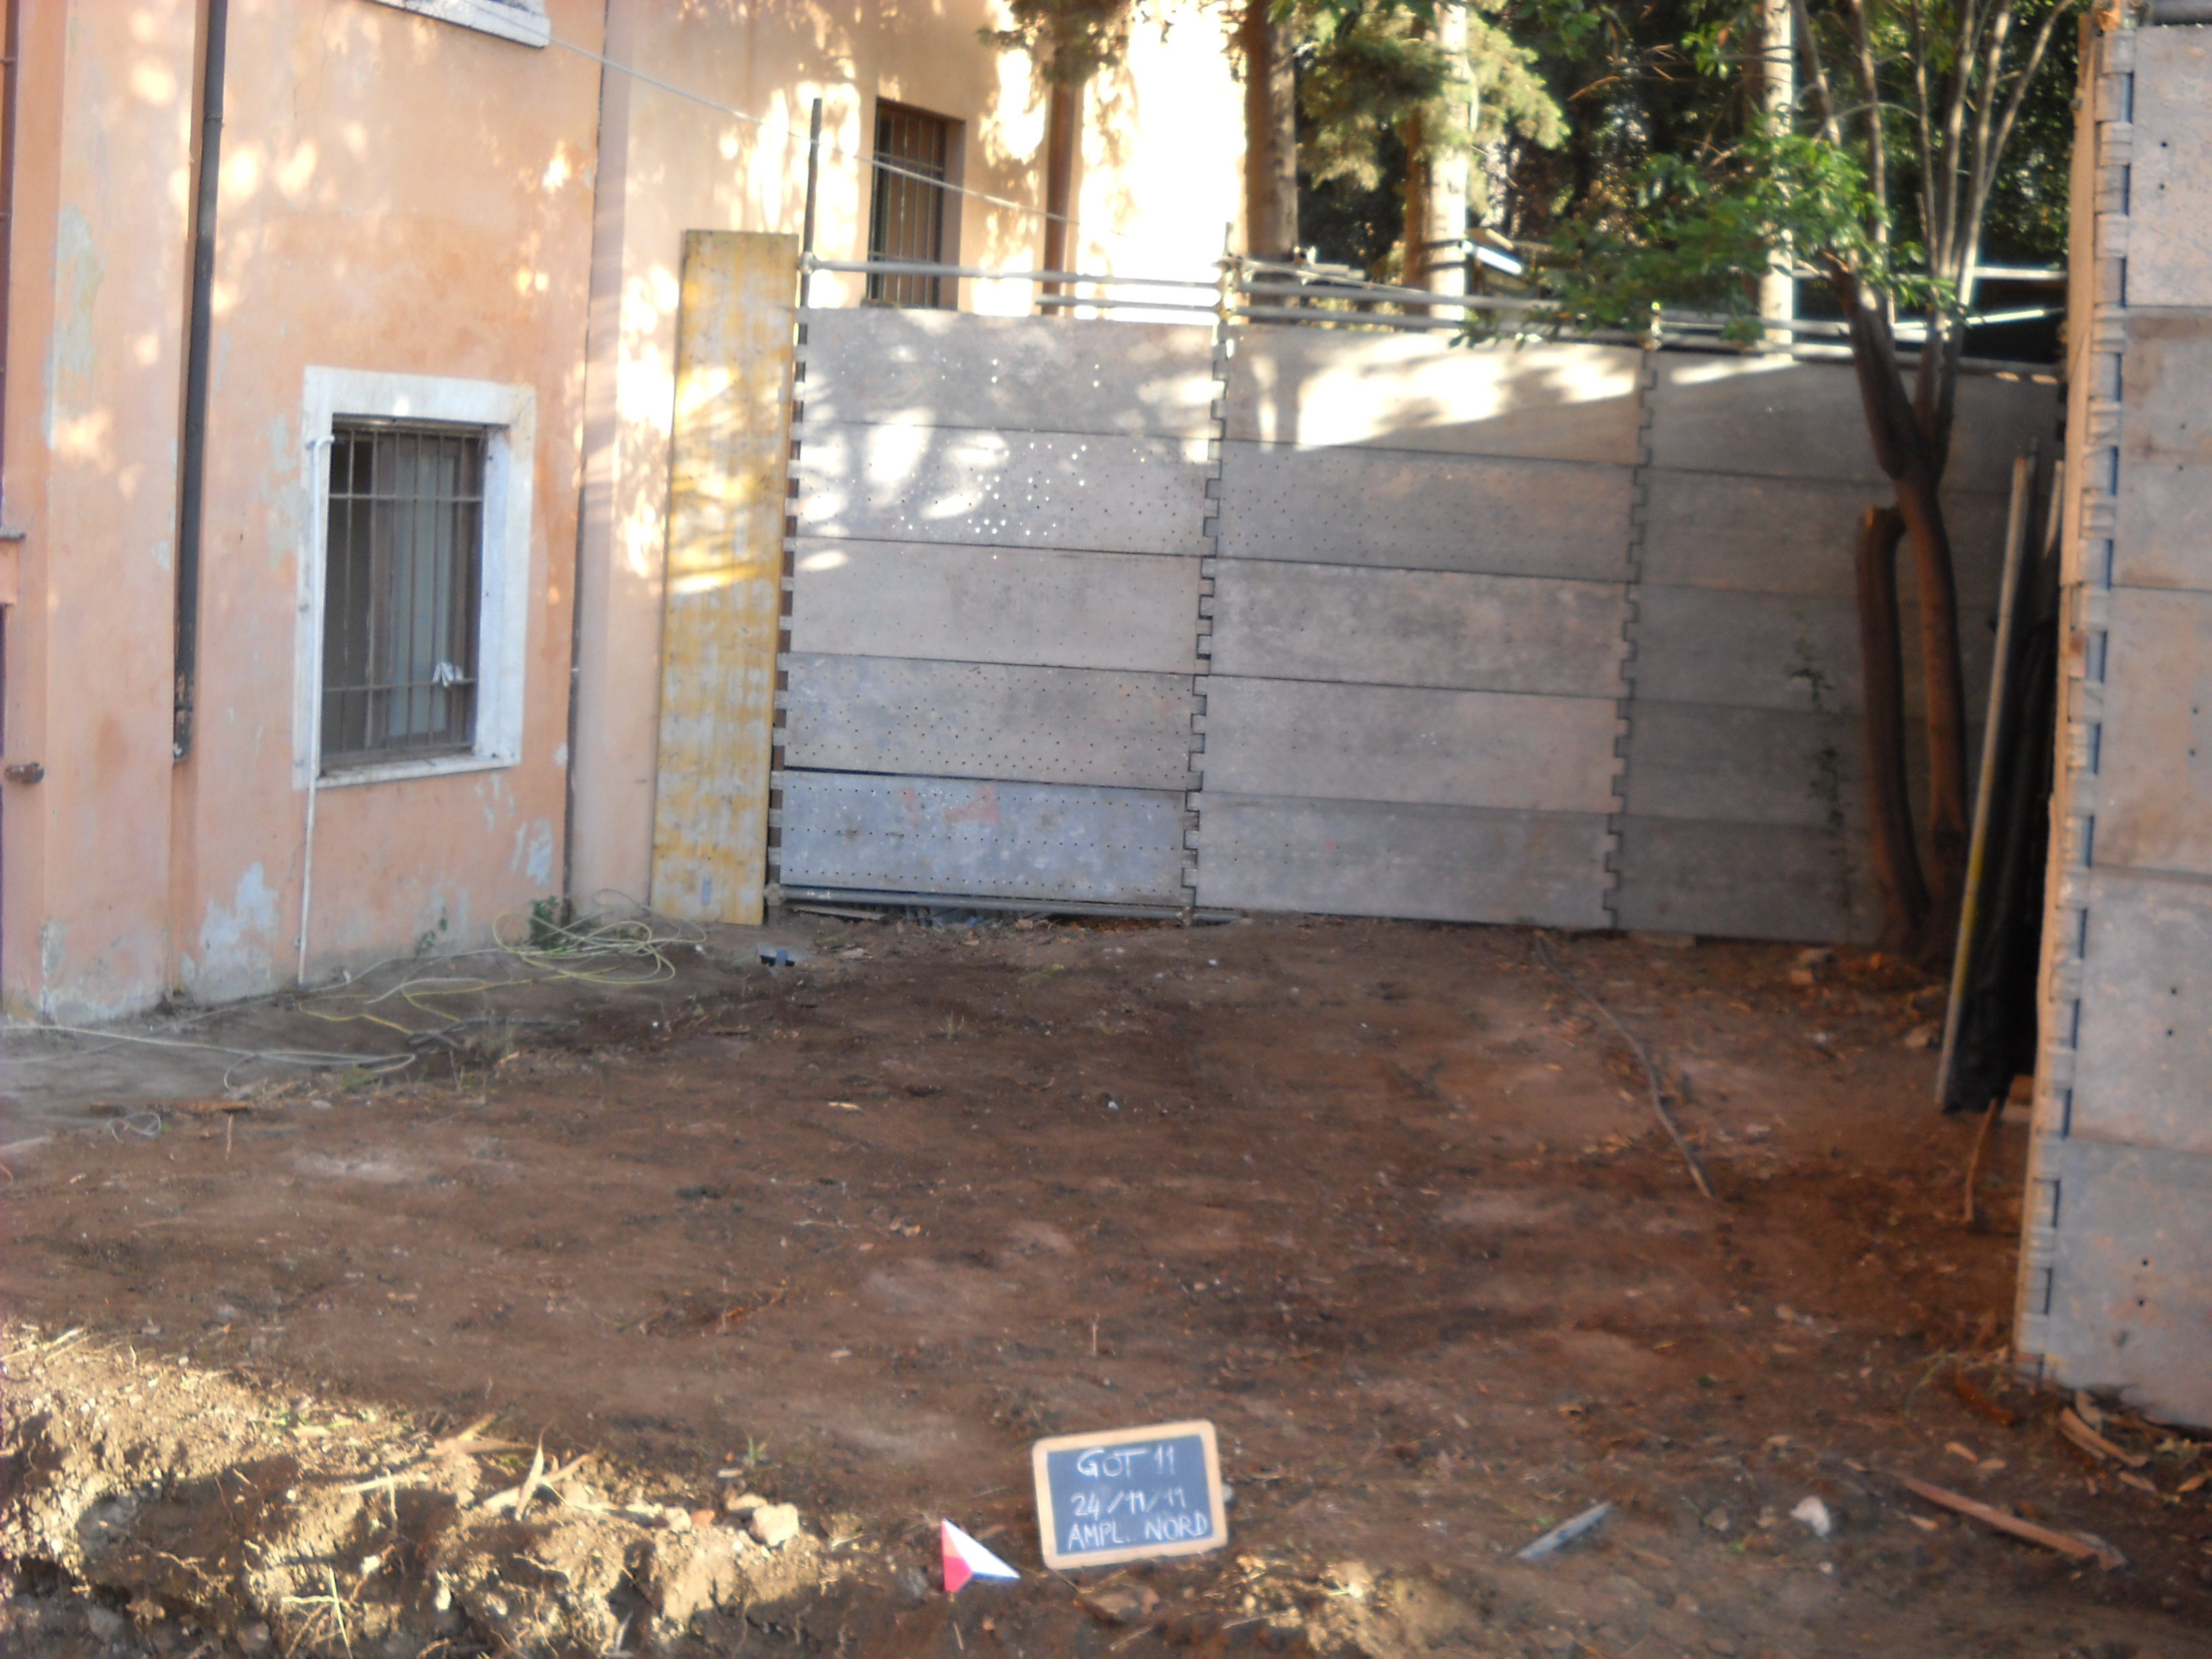
\includegraphics[width =0.5\textwidth]{catacom_1111.JPG}
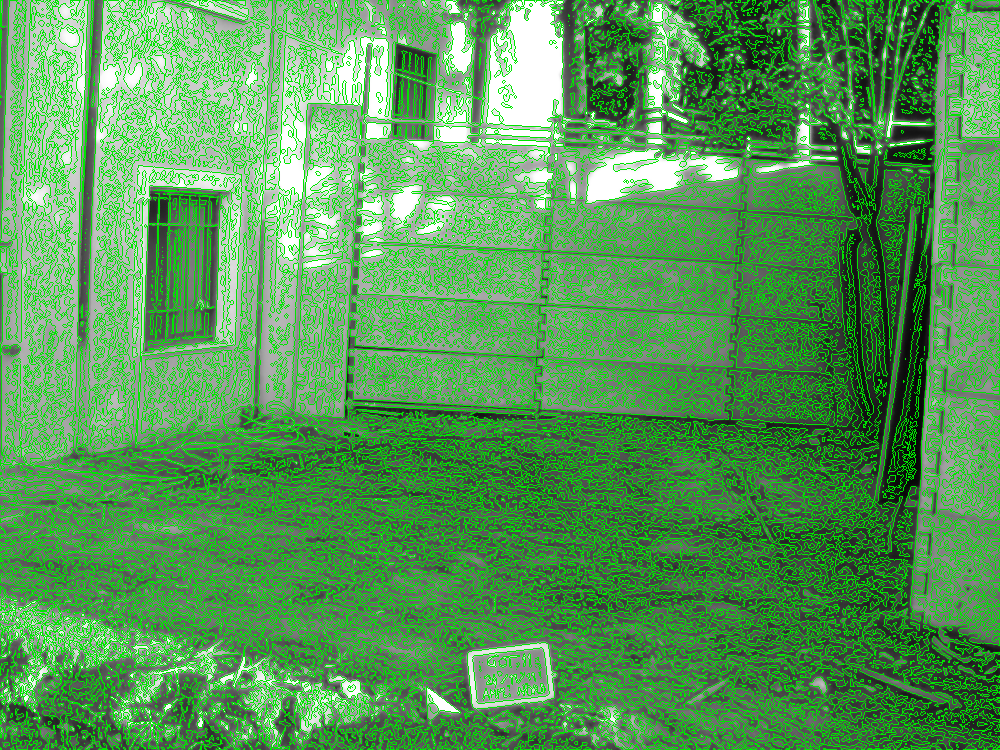
\includegraphics[width =0.5\textwidth]{catacom_1111_adaptive_cont.png}
\caption{Grabungsfoto im Original sowie nach der Anwendung der Konturerkennung.}
\label{fig:adaptivecont}
\end{figure}
%Zweispurigkeit der Ansätze: iterativ und adaptiv. Erklären warum.
%\verb|rect_detect| als Finale, in dem die beiden Ansätze wieder zusammengeführt werden
Als nächstes müssen unter diesen Konturen die ausgewählt werden, die als Tafel in Frage kommen. Dazu wird die Tatsache genutzt, dass Tafeln auf den Fotos als Rechtecke abgebildet werden. Durch ihre Lage zur Kamera können sie zu einem gewissen Grad davon abweichen, grundsätzlich bleibt diese Form aber erhalten. Andere Rechtecke kommen zwar vor, wie Plakate, Fenster, Türen, Ziegel und Fliesen, unterscheiden sich jedoch meist in der tatsächlichen Form oder können im Zweifelsfall bei der späteren Texterkennung ausgeschlossen werden. Dementsprechend geht es in der weiteren Tafelerkennung darum, Rechtecke zu finden und diese durch verschiedene weitere Kriterien so zu sortieren, dass alle Tafeln und möglichst nur Tafeln erkannt werden. Das wird in mehreren Schritten erreicht:
Zunächst wird die Fläche der Konturen berechnet. Genutzt wird hierfür die OpenCV-Funktion \verb|cv2.contourArea|. Ist die Fläche zu klein, wird die Kontur aussortiert. Als Grenzwert wird hier die Kantenlänge der längsten Kante des Bildes genommen, damit bei höherer Auflösung weiterhin korrekt sortiert werden kann(Vgl. Abb. \ref{fig:adaptivecontsize}). Eine Größenbegrenzung ist sinnvoll, da die Tafeln in der Regeln eher prominent im Bild zu sehen sind. Sollte tatsächlich eine Tafel durch dieses Kriterium aussortiert werden, wäre der Text darauf nicht mehr lesbar und somit ohnehin nicht interessant für die weitere Verarbeitung.
\begin{figure}[h!]
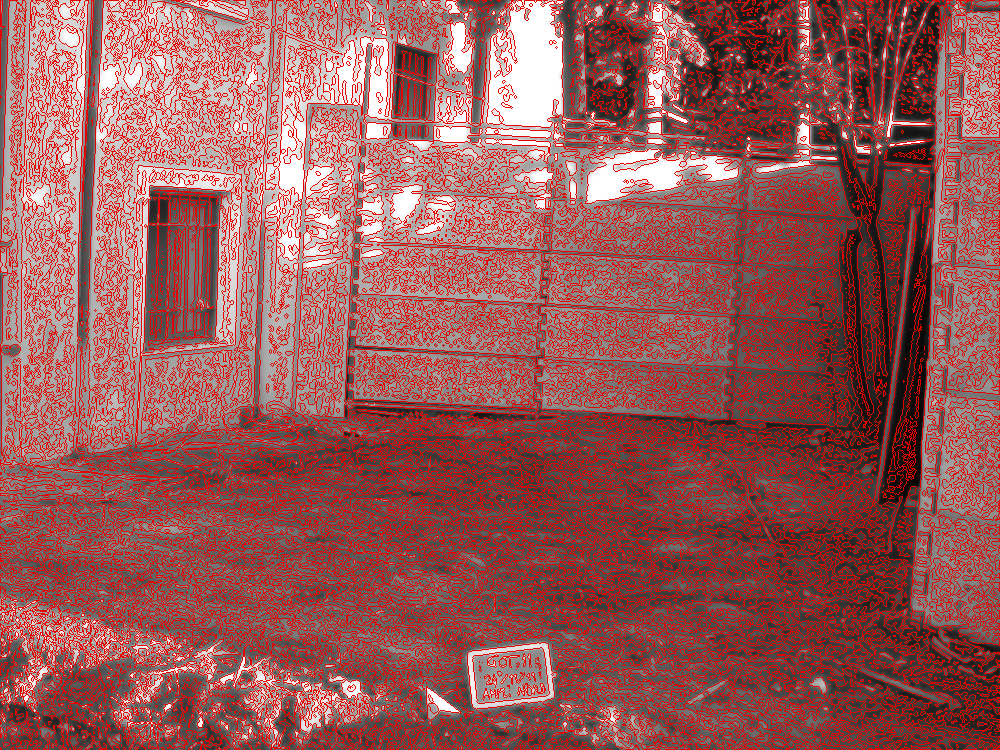
\includegraphics[width =0.5\textwidth]{catacom_1111_adaptive_contred.png}
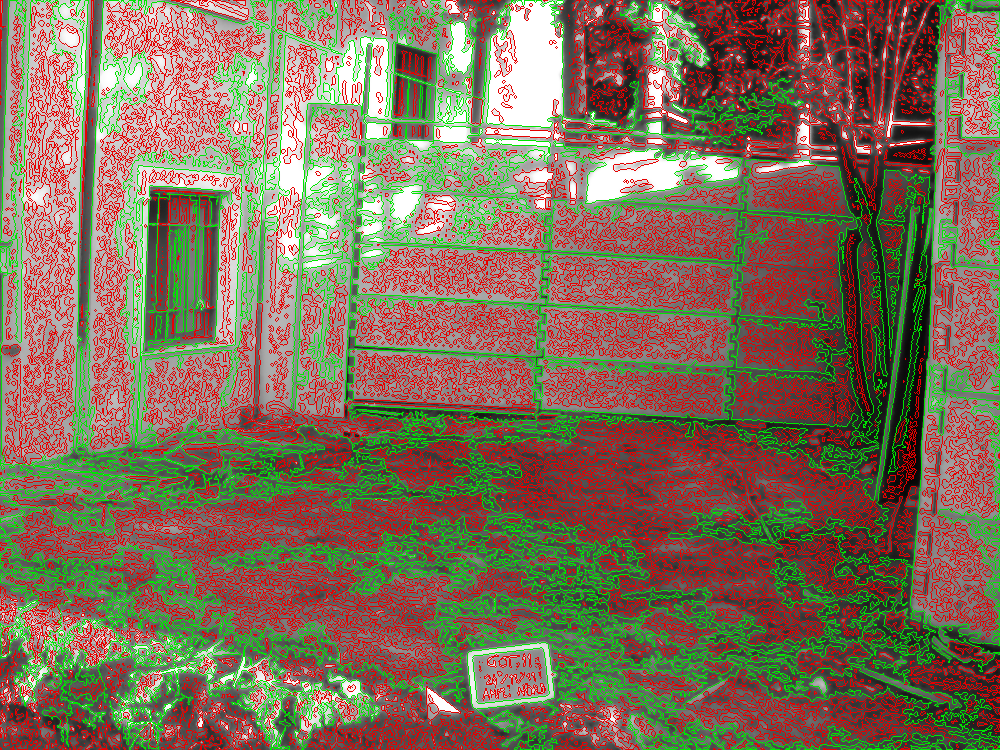
\includegraphics[width =0.5\textwidth]{catacom_1111_adaptive_bigcont.png}
\caption{Konturen vor und nach der Selektion nach Fläche.}
\label{fig:adaptivecontsize}
\end{figure}

Der nächste Schritt besteht darin, durch \verb|cv2.minAreaRect| das kleinstmögliche Rechteck um die Kontur zum bilden (Vgl. Abb. \ref{fig:adaptiverectangles}).
\begin{figure}[h!]
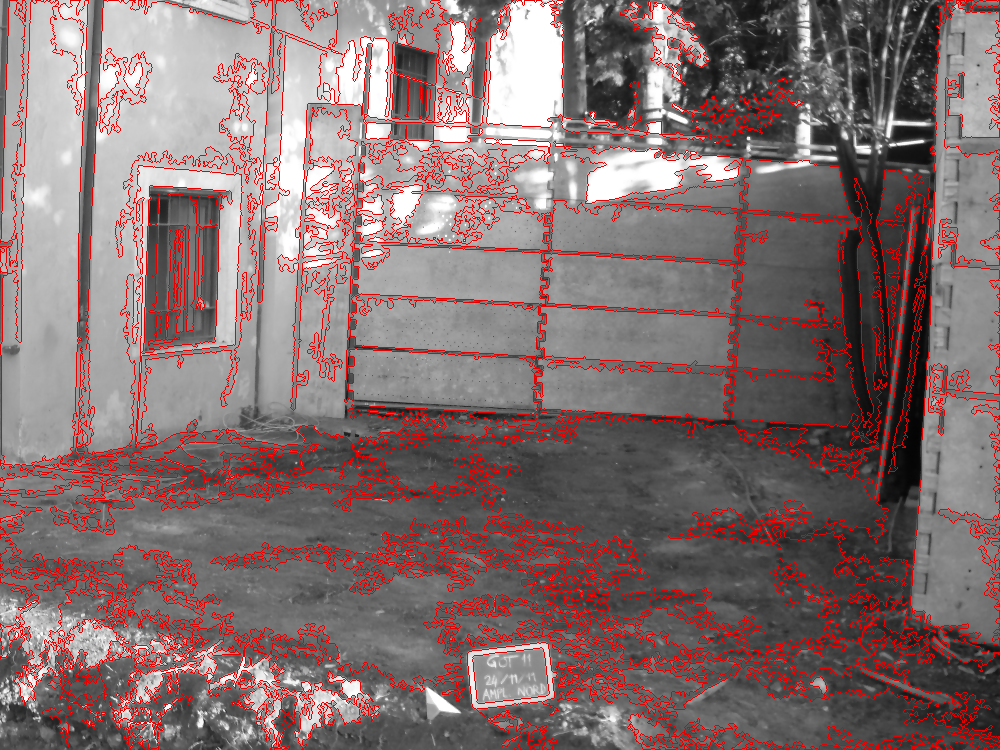
\includegraphics[width =0.5\textwidth]{catacom_1111_adaptive_bigcontred.png}
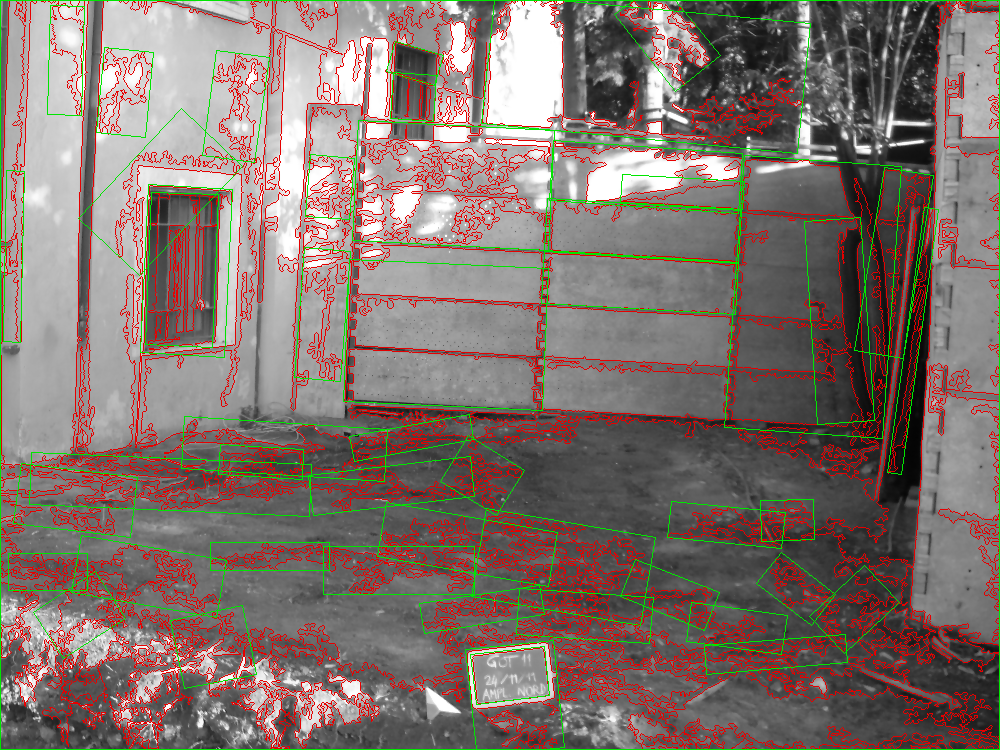
\includegraphics[width =0.5\textwidth]{catacom_1111_adaptive_allrects.png}
\caption{Konturen ohne und mit Rechtecken.}
\label{fig:adaptiverectangles}
\end{figure}

Anschließend werden die bereits berechneten Flächen der Konturen mit denen der kleinstmöglichen Rechtecke verglichen. Die Annahme: Nähert sich der Flächeninhalt der Kontur dem des Rechtecks an, handelt es sich bei der Kontur selbst wahrscheinlich um ein Rechteck. Dabei hat sich als Grenzwert bewährt, dass die Fläche der Kontur 85\% der Fläche des Rechtecks betragen sollte. Ebenfalls ausgeschlossen wird ein Rechteck, wenn es die Fläche des gesamten Bildes ausmacht, da teilweise, wie auch bei diesem Beispiel, der Rand des Bildes als Kontur erkannt werden kann (Vgl. Abb. \ref{fig:adaptivrect}).
\begin{figure}[h!]
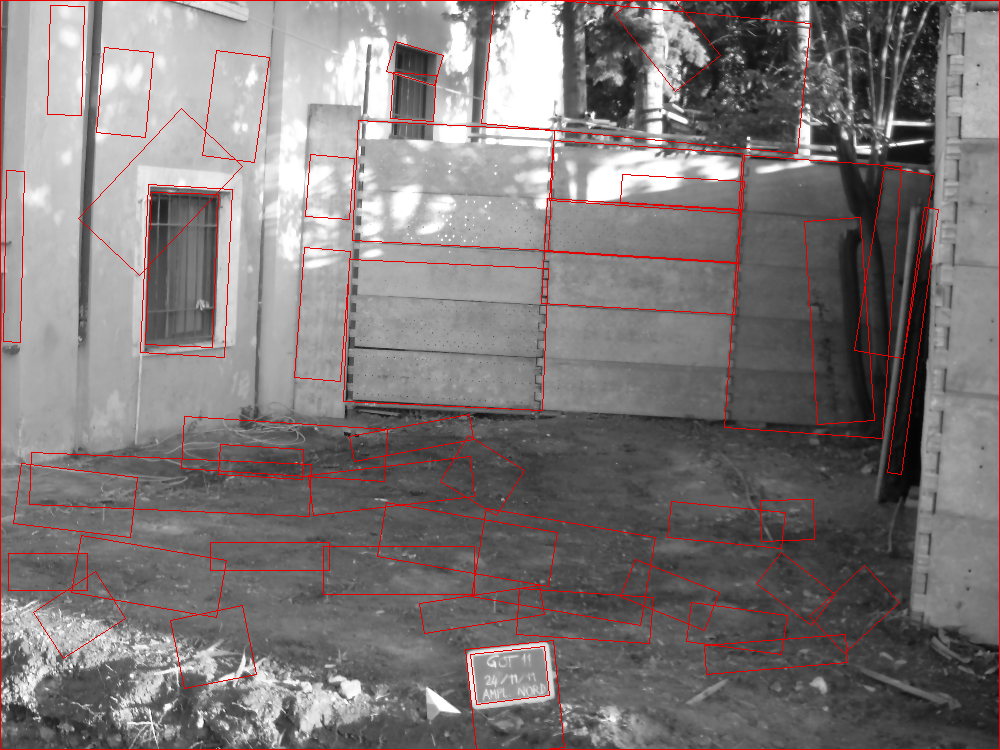
\includegraphics[width =0.5\textwidth]{catacom_1111_adaptive_allrectsred.png}
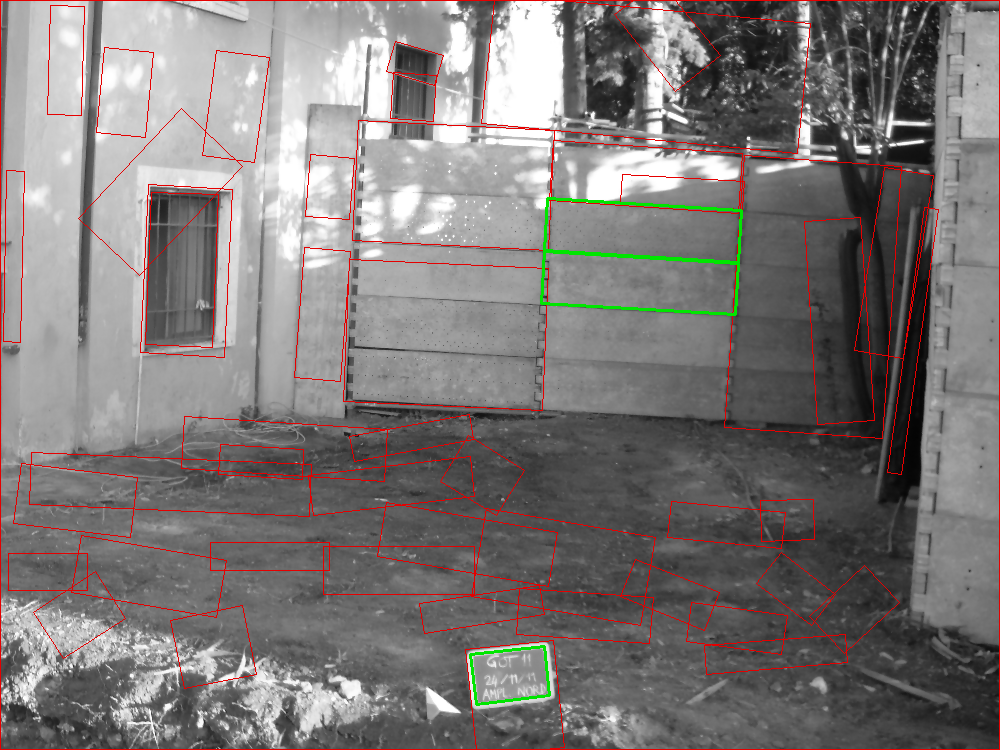
\includegraphics[width =0.5\textwidth]{catacom_1111_adaptive_rectarea.png}
\caption{Rechtecke aller Konturen und jene derer mit annähernd rechteckiger Fläche.}
\label{fig:adaptivrect}
\end{figure}

Als letztes Kriterium wird das Seitenverhältnis herangezogen. Im Programm besteht die Möglichkeit, vor der Untersuchung aller Bilder ein Template zu hinterlegen, auf dem eine Tafel gut und eindeutig zu sehen ist. Aus diesem Template wird das Seitenverhältnis der Tafel berechnet. Findet dieser Schritt nicht statt, wird ein maximales Seitenverhältnis von 2:1 angenommen, da Tafeln selten in länglichen Formaten zu finden sind\footnote{Sollte das Format einer Tafel doch einmal von dieser Annahme abweichen, lassen sich hier problemlos Anpassungen vornehmen.}. Mit einer deutlichen, Toleranz von 30\% in jede Richtung wird das Seitenverhältnis der verbliebenen Rechtecke mit dem des Templates verglichen. Sind die Werte sich ähnlich genug, wird das Rechteck als Tafel interpretiert und gilt als das Ergebnis des Algorithmus (Vgl. Abb. \ref{fig:aspectratio}).
\begin{figure}[h!]
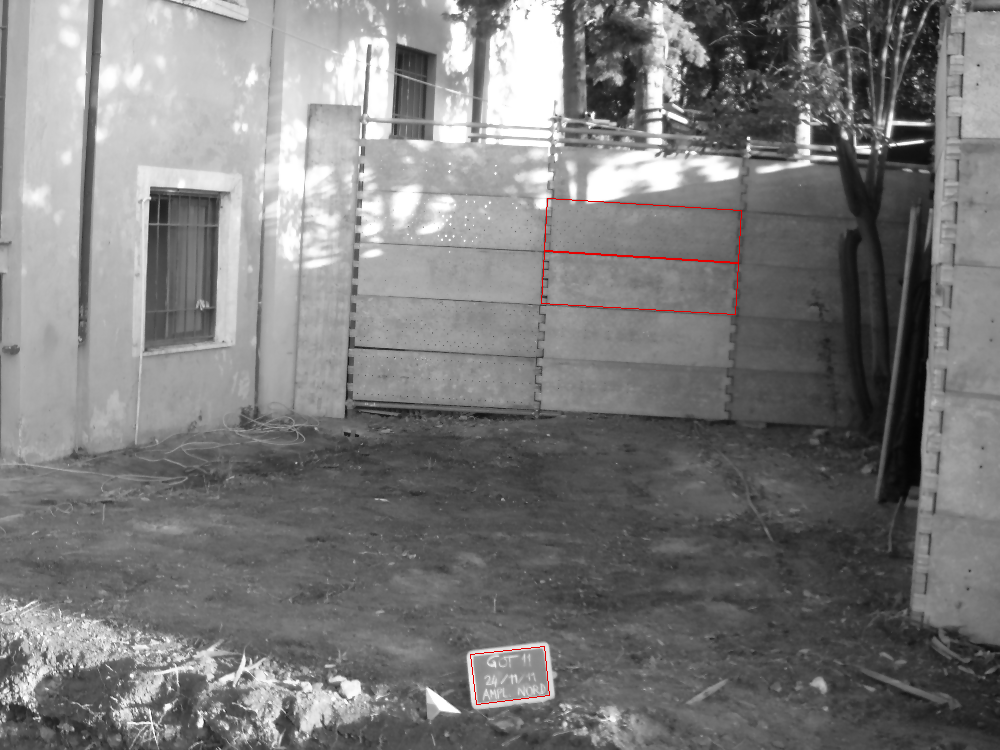
\includegraphics[width =0.5\textwidth]{catacom_1111_adaptive_rectareared.png}
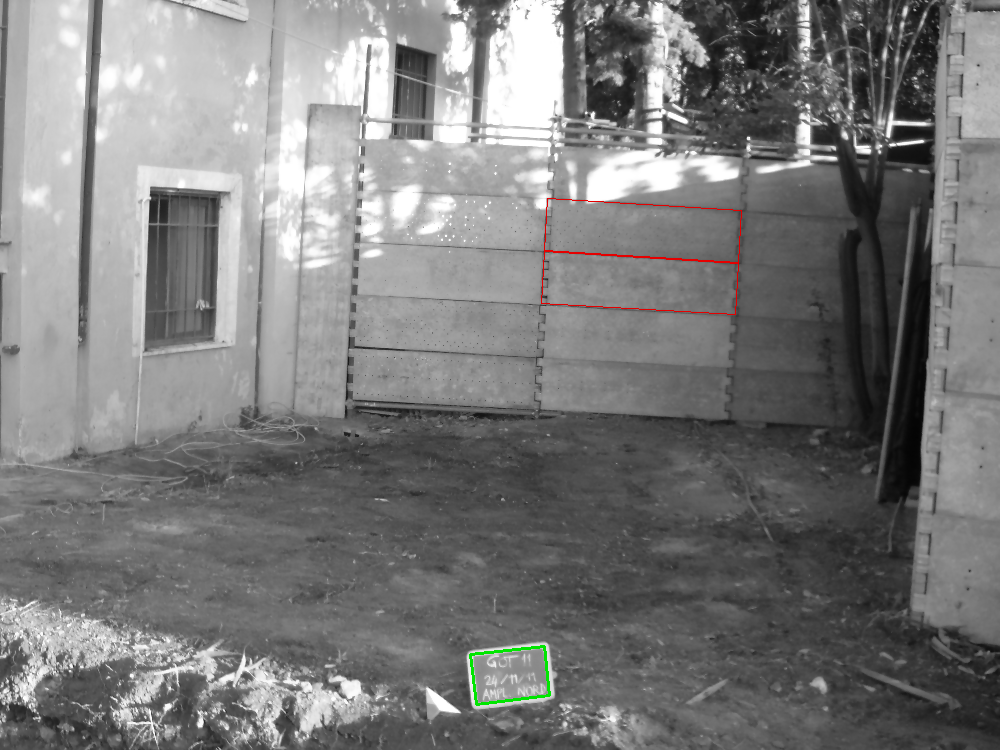
\includegraphics[width =0.5\textwidth]{catacom_1111_adaptive_aspectratio.png}
\caption{Die bisher verbliebenen Rechtecke und die mit dem richtigen Seitenverhältnis.}
\label{fig:aspectratio}
\end{figure}
 
\subsection{Cropverfahren}

Durch die vorhergehende Rechtecksdetektion sind die Positionen der Tafeln bekannt. Der nächste Schritt besteht darin, die Tafeln aus dem Gesamtbild auszuschneiden, damit diese Ausschnitte für die Texterkennung genutzt werden können. Auch die perspektivischen Verzerrungen der Tafeln ausgeglichen werden müssen. Für diesen Ausgleich müssen die Eckpunkte der Tafeln bestimmt und das durch sie definierte Viereck auf die Fläche eines Rechtecks übertragen werden.
Auch hier haben sich wieder zwei Verfahren ergeben, von denen eines effizient arbeitet, während das zweite stärker auf das Entzerren der Bilder abzielt (Vgl. Abb. \ref{fig:flowchartcrop}).
\begin{figure}[h!]
\centering
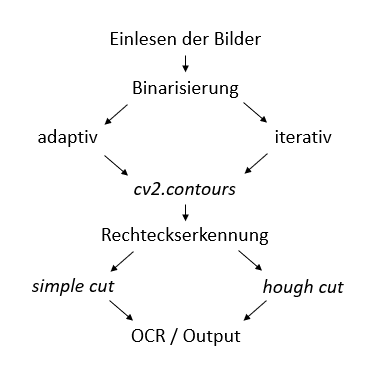
\includegraphics[width =0.5\textwidth]{flowchart_cont_crop.PNG}
\caption{Flowchart Crop-Verfahren.}
\label{fig:flowchartcrop}
\end{figure}
%Was ist die Aufgabe beim Crop?
%Worin liegen hier die Schwierigkeiten?
%Auch hier wieder Zweispurigkeit der Ansätze erklären

\subsubsection{Simple Crop}

Ein Weg, die Tafeln aus den Bildern auszuschneiden, besteht darin, die kleinstmöglichen Rechtecke aus dem Detektionsverfahren als Basis für den Ausschnitt zu nutzen. Basierte die Detektion auf dem adaptiven Ansatz, musste zunächst das Rechteck auf die ursprüngliche Bildgröße skaliert werden, da für die weitere Verarbeitung die Originalbilder mit der höheren Auflösung verwendet wurden. Zu diesem Zweck wurde das Verhältnis aus der Größe des Originalbildes und der des skalierten Bildes gebildet. Multipliziert man dieses Verhältnis mit den vier Kennzahlen der Rechtecke (X- und Y-Koordinate des Mittelpunktes sowie Breite und Höhe) wird das Rechteck passend skaliert. Als letzter Schritt wurden aus diesen Werten, unter Einbezug der Rotation des Rechtecks, die Eckpunkte berechnet.  Neben den so erhaltenen Ausgangskoordinaten mussten aber auch Zielkoordinaten erzeugt werden, auf die das Rechteck projiziert wird. Diese wurden ebenfalls dem Detektionsrechteck entnommen, indem Höhe und Breite als Maße für das Projektionsziel genutzt wurden.
Für die Transformation des Ausgangsrechtecks auf das Zielrechteck wurde mittels \verb|cv2.tafelcrop| die Transformationsmatrix erzeugt (\cite{cvtransform}). Die eigentliche Transformation erfolgte dann durch \verb|cv2.warpPerspective| (Vgl. Abb. \ref{fig:aspectratio}).
Der so erzeugte Tafelausschnitt wurde anschließend auf 1000 Pixel skaliert, was in der Regel eine Vergrößerung darstellt, um eine einheitliche Größe zu gewährleisten und zu kleine Ausschnitte zu vermeiden. Außerdem wurde das Bild um 90 \degree rotiert, wenn die Höhe die Breite übertraf, um nur Ausschnitte im Querformat zu erhalten.

\begin{figure}[h!]
\centering
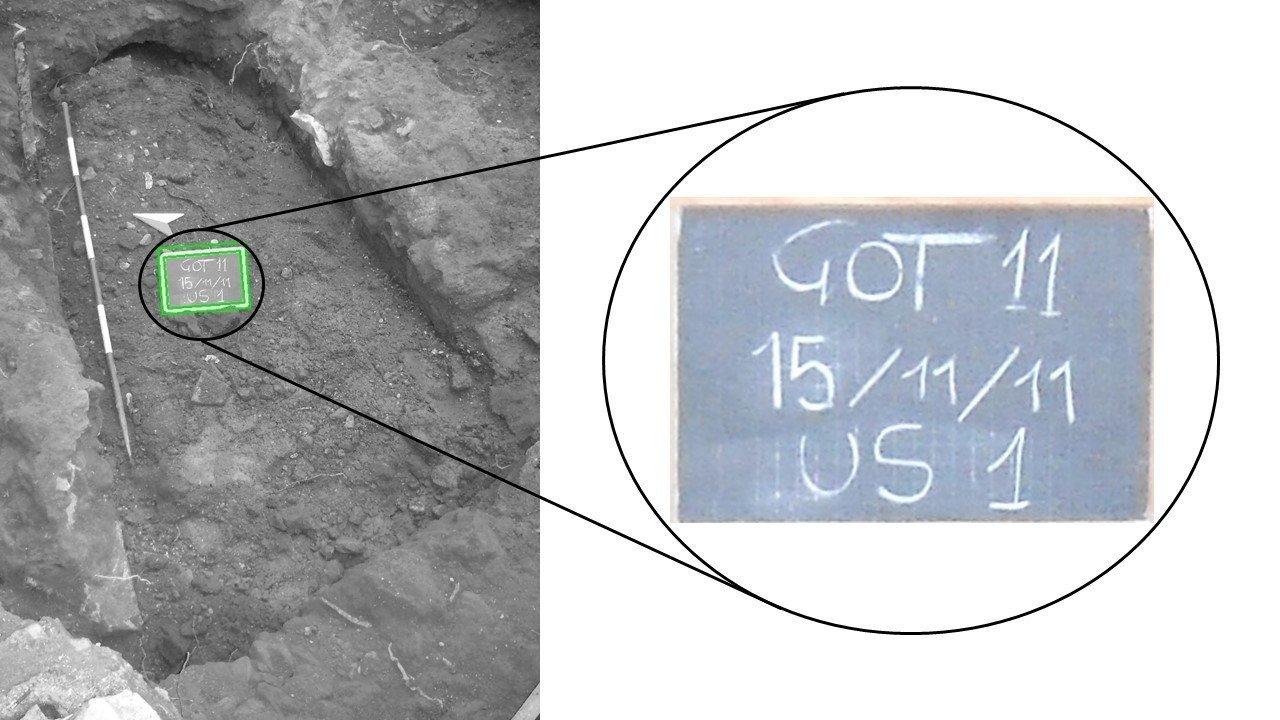
\includegraphics[width =0.75\textwidth]{Tafel Zoom.jpg}
\caption{Eine Tafel vor und nach dem Ausschneiden.}
\label{fig:tafelcrop}
\end{figure}

\subsubsection{Hough Crop}

%Was ist die Idee?
%Wie wurde sie umgesetzt?
%Wo liegen die Probleme?
Durch unterschiedlichen Perspektiven, aus denen die Fotos aufgenommen wurden, ist die beschriftete Seite der Tafeln nicht immer frontal der Kamera zugewendet. \verb|Simple Crop| ist nicht geeignet, um die daraus resultierende Verzerrung auszugleichen (Vgl. Abb. \ref{fig:parallelogramm}). 

\begin{figure}[h!]
\centering
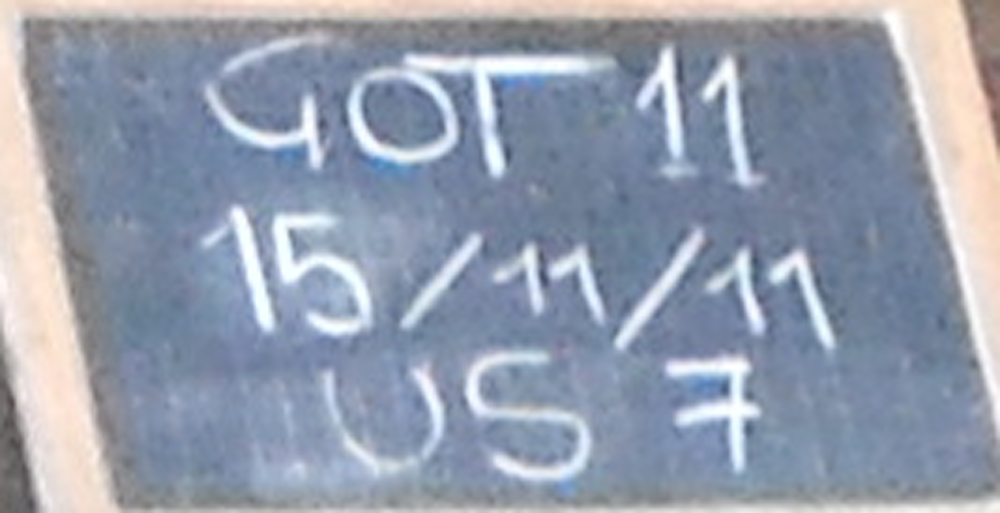
\includegraphics[width =0.5\textwidth]{catacom_1073_0.png}
\caption{Diskrepanz zwischen den Eckpunkten der gefundenen Rechtecke und den Eckpunkten der Tafel.}
\label{fig:parallelogramm}
\end{figure}

Daher wurde ein zweiter Ansatz entwickelt, um dieses Problem zu beheben. Ziel war es hier, statt der Eckpunkte der gefundenen Rechtecke die Eckpunkte der Tafel für das Cropverfahren zu nutzen. Diese mussten also zunächst gefunden werden. Das kann erreicht werden, indem die Seiten der Tafeln durch Kantendetektion ermittelt und im Anschluss deren Schnittpunkte berechnet werden \cite{qixiangye}.
Zunächst musste dazu ein passender Bildausschnitt gewählt werden. Auf den Tafeln befinden sich viele Objekte, die lange gerade Kanten aufweisen. Nach der Detektion zu entscheiden, welche davon Teil einer Tafel sind und welche nicht ist komplex und würde die gesamte Problematik der Detektion neu aufwerfen. Gleichzeitig konnten auch die detektierten Rechtecke nicht verwendet werden, da hier Teile des Rahmens abgeschnitten sein können. Daher wurden die Rechtecke um den Faktor 1,3 vergrößert und mittels \verb|simple crop| ausgeschnitten (\ref{fig:tafelrechteck}.

\begin{figure}[h!]
\centering
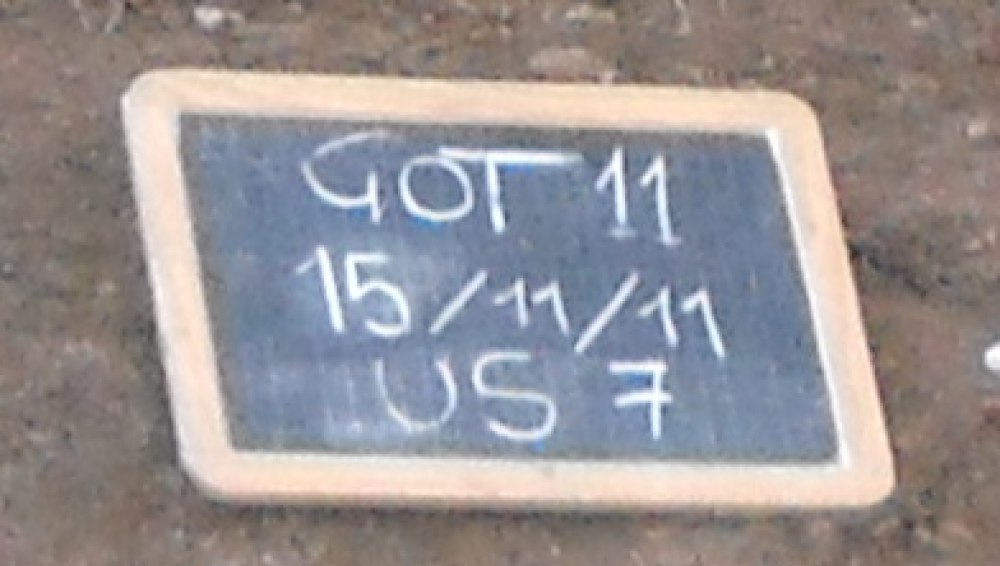
\includegraphics[width =0.5\textwidth]{1073_new_rect.png}
\caption{Bildausschnitt für Hough Crop, basierend auf dem vergrößerten Tafelrechteck.}
\label{fig:tafelrechteck}
\end{figure}

Diese Bildausschnitte wurden mit mehreren Filtern bearbeitet, um das meist stark vorhandene Rauschen zu reduzieren. Es folgte die Umwandlung in ein Graustufenbild, das normalisiert wurde. Beim Prozess der Normalisierung werden Farbskalen, in diesem Fall also die Graustufen, auf ihre maximalen Werte gestreckt. Der niedrigste wird also auf 0, der höchste auf 255 gesetzt und alle Werte dazwischen entsprechend angepasst. Auf die normalisierten Bilder wurde die \textit{Canny Edge Detection} (Kantenerkennung) angewendet \cite{cannyedge}. Dieser Algorithmus berechnet die Gradienten der einzelnen Pixel, wodurch Kantenverläufe im Bild erkennbar werden. Auf diese wird eine \textit{non-maximum supression} angewendet, d.h., die Gradienten der Pixel werden mit ihren Nachbarn verglichen und jeweils nur das Maximum weiterverwendet. Die Kantenstärke wird somit auf die Breite von einem Pixel reduziert. Aus den so erhaltenen Gradienten werden mittels zweier Schwellwerte durch Hysterese die gewünschten Kanten bestimmt: Enthält ein Pixel einer Kante den zweiten, höheren Schwellwert, gilt sie als eine der gesuchten Kanten. Von dort ausgehend werden alle Pixel der Kante, die den niedrigeren Schwellwert übertreffen, ebenfalls als Teil dieser Kante.
Dieses Gradientenbild wiederum wurde mittels Hough\footnote{Gesprochen: [h\textturnv{}f]}-Transformation \cite{houghpatent} einer Linienerkennung unterzogen. Die vorher detektierten Kanten, die einen beliebigen Verlauf nehmen können, wurden also jetzt darauf geprüft, ob sie eine gerade Linie bilden. Das erfolgt, indem mit der hesseschen Normalform jede mögliche Gerade durch jeden Kantenpunkt berechnet wird. Jeder Kantenpixel, durch den die Geraden verlaufen, erhält einen \textit{upvote}, es wird also ein Zähler inkrementiert. Durch die Bereiche mit den meisten \textit{Upvotes} laufen die gesuchten Linien auf dem Bild. Ist eine Linie gefunden, ist sie wahrscheinlich Teil des Rahmens der Tafel und somit für die Erkennung der Eckpunkte relevant.
Im nächsten Schritt wurden die Geraden mit dem Bildrahmen geschnitten. Die Schnittpunkte wurden als neue Endpunkte des Liniensegments für die weiteren Berechnungen genutzt. Die Endpunkte wurden, entsprechend ihrer Position im Bild, den vier Ecken zugeteilt. Anschließend wurden die Schnittpunkte der Linien untereinander berechnet, aber nur, wenn sie 1) nicht in die gleiche Richtung und 2) nicht diagonal durchs Bild verliefen. Beide Kriterien konnte durch die Einordnung der Eckpunkte bestimmt werden. Damit war sichergestellt, dass nur Linien miteinander geschnitten wurden, die annähernd senkrecht zueinander verlaufen, wie es bei den Tafelrändern der Fall ist.
Die Gruppe der Schnittpunkte wurde wiederum in die vier Ecken aufgeteilt. In jeder Ecke wurde jetzt der Punkt bestimmt, der am weitesten Richtung Bildmitte liegt. Dieser wurde als der wahrscheinlichste Eckpunkt angenommen.
Das weitere Verfahren entsprach dem des \verb|simple crop|-Ansatzes: Mit den Eckpunkte wurde eine Transformationsmatrix berechnet, durch die der Bildausschnitt innerhalb der vier Eckpunkte auf eine Rechtecksform übertragen werden konnte.


\subsection{Texterkennung}

Im folgenden Abschnitt wird der zweite Aspekt der Verarbeitung von Grabungsfotos vorgestellt: Die Texterkennung oder \textit{optical character recognition} (OCR). Da die Vorbereitung der Bilder für das Gesamtergebnis von großer Bedeutung ist, wird zunächst das \textit{Preprocessing} behandelt. Im Anschluss wird die eigentliche Texterkennung mit Tesseract vorgestellt.
Folgende Probleme müssen bei der Texterkennung adressiert werden: (1) Komplexität der Szene, (2) Beleuchtungsverhältnisse, (3) Rotation des Textes relativ zur Kamera, (4) Unschärfe, (5) Größe und Format der Textfelder, (6) Neigungswinkel des Textes relativ zur Kamera, (7) Schriftart, (8) Mehrsprachigkeit, (9) perspektivische Verzerrungen \cite{hamad}. In diesem Falle wurde allen Aspekten, die der Textdetektion gelten (1, 5), geringeres Gewicht beigemessen, da die Tafeln bereits als die Grenzen des beschriebenen Areals betrachtet werden konnten. Die Neigung und die Schiefe der Buchstaben relativ zur Kamera (3,6,9) wurden bereits beim Cropverfahren entsprechend der Möglichkeiten ausgeglichen. Beleuchtung, Unschärfe und Rauschen waren Teil des Preprocessings (2.4), die sprachbezogenen Punkte (7,8) wurden im Rahmen der eigentlichen Texterkennung adressiert.

\subsubsection{Preprocessing}

Das Preprocessing für die Texterkennung folgte gängigen Verfahren\footnote{Warum übliche Schritte im Preprocessing, wie das Thresholding, hier unterblieben, wird im weiteren Verlauf dieser Arbeit ausführlich diskutiert werden.} \cite{jenilshah}, \cite{sumedhahallale}. Zunächst mussten die Bilder in Graustufen umgewandelt werden. Nacheinander wurden zwei Filter angewendet, \verb|cv2.GaussianBlur| und \verb|cv2.fastNlMeansDenoising|. Damit sollten die Störeffekte durch verwischte Kreide auf der Tafel ausgeglichen werden. Das Bild wurde invertiert, sodass die eigentliche weiße Kreide schwarz dargestellt und der Hintergrund hell wurde, was den Empfehlungen für Tesseract entspricht \cite{tesseractoptimum}. Der letzte Schritt bestand in der Normalisierung der Bilder. Alle diese Schritte wurden auf das Grundbild sowie die daraus extrahierten 3 Farbkanäle angewendet.

\subsubsection{OCR}

Pro gefundener Tafel waren jetzt vier Bilder vorhanden, die der Texterkennung unterzogen werden konnten. Für jedes dieser Bilder wurde diese doppelt ausgeführt: Einmal mit \verb|image_to_string| und einmal mit \verb|image_to_boxes|. Ersteres liest den Text Zeilenweise ein, letzteres jeden Buchstaben einzeln. \verb|Image_to_string| wurde zusätzlich auf das um 180\degree rotierte Bild angewendet, um die Orientierung zu ermitteln: Die Ergebnisse der Texterkennung beider Orientierung wurden, nach der Bereinigung von Leerzeichen und Zeilenumbrüchen, anhand der Länge miteinander verglichen. Die Version, bei der mehr Text gefunden wurde, wurde als korrekt orientiert angenommen. Eine solche Funktion ist zwar in Tesseract bereits grundsätzlich implementiert, da die Texterkennung hier aber ohnehin unter erschwerten Bedingungen und ohne erkennbare Wörter stattfand, wurde auf diesen Ansatz zurückgegriffen\footnote{U.a. liefert die Funktion image\_to\_osd von Pytesseract die Orientierung des gefundenen Textes. Für die Anwendung derselben befindet sich auf den Tafeln zu wenig Text.}.
Die Ergebnisse der beiden Pytesseract-Funktionen aus den je vier Bildern wurden im Anschluss untereinander verglichen. Der längste gefundene Text wurde als Ergebnis übernommen.
Beide Befehle wurden mit folgender Konfiguration ausgeführt: (1) Es wurde eine Whitelist verwendet, die auf das Schema der Tafeln zugeschnitten wurde. Gelistet wurden die Ziffern \textit{0-9}, die Buchstaben \textit{G,O,T,U} und \textit{S} sowie das Sonderzeichen \textit{/}. (2) Als Sprache wurde ein eigenes Wörterbuch angegeben, das entsprechend der Tafeln nur wenige Worte enthält (\textit{US, GOT}. (3) Der \textit{OCR Engine Mode} (oem) wurde auf ein Neurales Netzwerk mit \textit{Long Short-term Memory}\cite{hochreitersepp} festgelegt. (4) Für die \texit{Page Segmentation} (psm) wurde ein vollautomatischer Modus, ohne weitere Vorgaben, gewählt.

%\subsection{Experimentelles}

%\subsection{Zusammenfassung}
%evtl zusammenfassen wie vorgegangen wurde, warum dieser Weg gut ist und was das Wichtigste Ergebnis ist
\subsection{Evaluation}